% 第 2 章 微分形式引论
\chapter{微分形式引论}

本章我们引入本书的基本思想之一——微分 1-形式. 后续章节将讨论 $k>1$ 的微分 $k$-形式. 我们首先考察各种必要的要素, 缓慢而系统地建立起 1-形式的概念. 第 1 节引入笛卡尔坐标函数, 它在准确理解 1-形式是什么方面扮演着出人意料的角色, 并在 1-形式的记号中发挥作用.

第 2 节讨论流形、切空间与向量场, 其详细程度足以让你对它们是什么有一个良好的直觉认识, 而更严格的数学处理留待第 10 章. 第 3 节我们回到你在向量微积分中熟悉的方向导数. 向量微积分中方向导数通常的定义方式需要为我们的目的稍作调整. 一旦完成这一调整, 就可以在标准欧几里得单位向量与微分算子之间做出一个相当令人惊讶的等同. 这一等价在本书后续内容中扮演核心角色.

最后在第 4 节定义微分 1-形式. 透彻理解微分 1-形式需要把各种概念汇集起来：向量空间与对偶空间、欧几里得向量与微分算子的等价、方向导数以及笛卡尔坐标函数. 所有这些数学思想在 1-形式定义中的汇聚, 正是本章的目标.

\section{坐标函数}

既然我们已经回顾了必要的预备知识, 就可以开始进入本课程真正的核心内容：微分形式. 在课程的前半部分, 在我们理解基本概念之前, 我们将在 $\mathbb{R}^n$ 上处理微分形式, 并以 $\mathbb{R}^2$ 和 $\mathbb{R}^3$ 为主要例子. 只有在我们对微分形式建立了一些直觉之后, 才讨论更一般流形上的微分形式. 你可以非常宽泛地把流形想成一个局部为欧几里得的空间——这意味着如果你足够仔细地观察一个流形的一小部分, 那么它基本上看起来就像某个 $n$ 的 $\mathbb{R}^n$.

目前我们只使用我们熟悉的老式笛卡尔坐标系. 我们将在后面讨论其他坐标系. 我们习惯于把 $\mathbb{R}^2$ 画成带 $x$ 轴和 $y$ 轴的平面, 如图 \ref{fig:2-1} 所示. 这里我们在 $xy$ 平面上画出了点 $(2,1)$、$(-4,3)$、$(-2,-2)$ 和 $(1,-4)$. 类似地, 我们习惯于把 $\mathbb{R}^3$ 画成带 $x$、$y$、$z$ 轴的空间, 如图 \ref{fig:2-2} 所示. 这里我们画出了点 $(2,3,4)$、$(-3,-4,2)$ 和 $(4,1,-3)$. 还要注意, 本书在画 $\mathbb{R}^3$ 时遵循``右手法则''约定.

\begin{figure}[htbp]
  \centering
  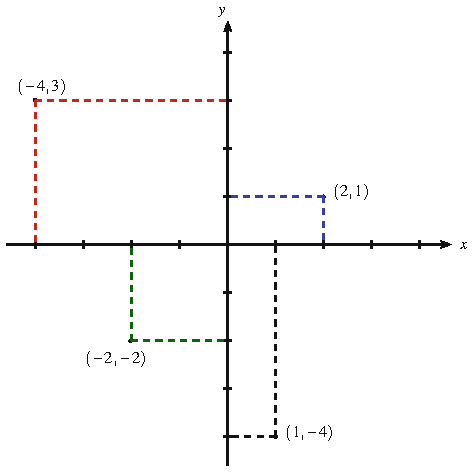
\includegraphics[width=0.562\linewidth]{images/vector/fig-2-1.pdf}
  \caption{$\mathbb{R}^2$ 的笛卡尔坐标系, 其中显示了点 $(2,1)$、$(-4,3)$、$(-2,-2)$ 与 $(1,-4)$.}
  \label{fig:2-1}
\end{figure}

\begin{figure}[htbp]
  \centering
  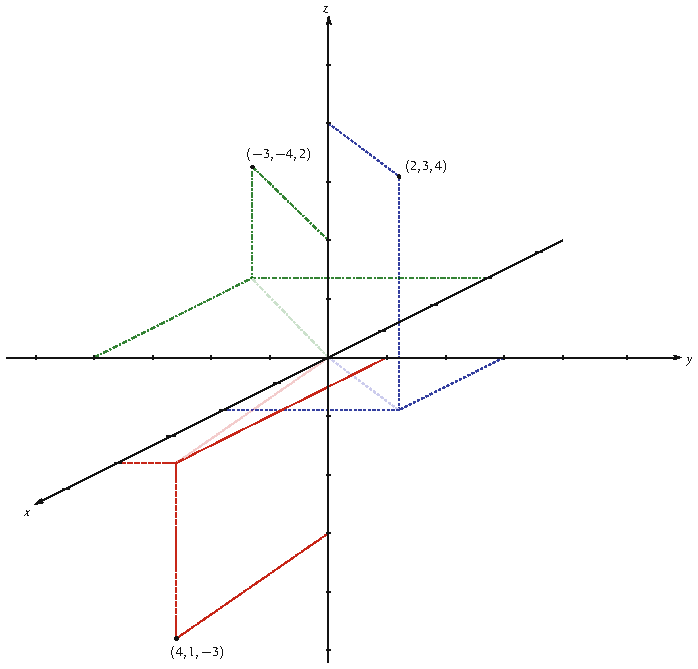
\includegraphics[width=0.932\linewidth]{images/vector/fig-2-2.pdf}
  \caption{$\mathbb{R}^3$ 的笛卡尔坐标系, 其中显示了点 $(2,3,4)$、$(-3,-4,2)$ 与 $(4,1,-3)$}
  \label{fig:2-2}
\end{figure}

注意 $\mathbb{R}^n$ 中点的记号与 $\mathbb{R}^n$ 中向量的记号之间的差别. 例如, $\mathbb{R}^2$ 或 $\mathbb{R}^3$ 中的点记为 $p=(x,y)$ 或 $p=(x,y,z)$, 其中 $x,y,z\in\mathbb{R}$；而 $\mathbb{R}^2$ 或 $\mathbb{R}^3$ 中的向量记为
\[
v=\binom{x}{y}\qquad\text{或}\qquad v=\begin{bmatrix}x\\y\\z\end{bmatrix},
\]
其中 $x,y,z\in\mathbb{R}$. 任意 $n$ 的 $\mathbb{R}^n$ 中的点与向量也类似地表示. 这里有一个微妙的区别, 在微积分课程中几乎总是被一带而过, 尤其是在多元微积分或向量微积分中, 然而这是一个非常重要的区别.
\begin{itemize}
  \item 我们把点的集合 $p=(x_1,x_2,\ldots,x_n)$（其中 $x_1,x_2,\ldots,x_n\in\mathbb{R}$）称为流形 $\mathbb{R}^n$.
  \item 我们把向量的集合 $v=\begin{bmatrix}x_1\\x_2\\\vdots\\x_n\end{bmatrix}$（其中 $x_1,x_2,\ldots,x_n\in\mathbb{R}$）称为向量空间 $\mathbb{R}^n$.
\end{itemize}

这一区别在微积分课程中被一带而过的原因之一是, 大多数微积分学生尚未修过线性代数课程, 还不知道什么是向量空间. 此外, 通过一点数学上模糊而不精确的处理, 确实可以不甚了解向量空间的技术定义就``做''向量微积分. 流形 $\mathbb{R}^2$ 和向量空间 $\mathbb{R}^2$ 看起来完全一样, 却是完全不同的空间. 它们已在图 \ref{fig:2-3} 中画出. 流形 $\mathbb{R}^2$ 包含点, 向量空间 $\mathbb{R}^2$ 包含向量. 当然, 就 $\mathbb{R}^2$、$\mathbb{R}^3$ 甚至 $\mathbb{R}^n$ 而言, 这些空间可以自然地等同. 也就是说, 它们实际上是相同的. 那么为什么做出这一区别如此重要呢？做出这一区别之所以重要有几个原因. 第一, 清楚地区分我们的空间将帮助我们更好地理解微分形式理论；第二, 当我们最终到达更一般的流形时, 大多数流形并不具有向量空间结构, 所以我们不想养成把流形也当作向量空间的坏习惯.

\begin{figure}[htbp]
  \centering
  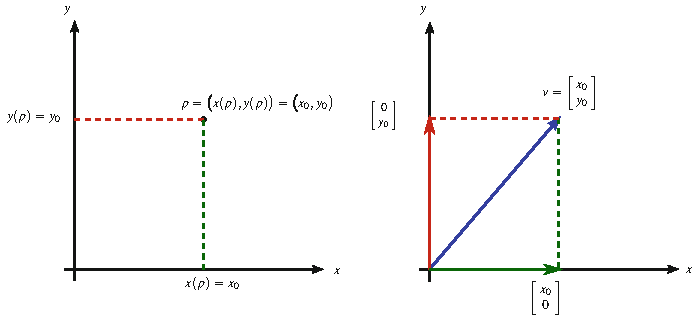
\includegraphics[width=0.938\linewidth]{images/vector/fig-2-3.pdf}
  \caption{流形 $\mathbb{R}^2$（左）与向量空间 $\mathbb{R}^2$（右）}
  \label{fig:2-3}
\end{figure}

现在让我们花一点时间回顾 $\mathbb{R}^2$ 和 $\mathbb{R}^3$ 上老式的普通函数. 我们将考虑实值函数, 它仅仅意味着值域（或陪域）是实数集 $\mathbb{R}$ 或实数集的某个子集. 来自 $\mathbb{R}^2$ 的实值函数最容易可视化, 因为它们可以在三维空间中作图. 考虑由 $f(x,y)=x^3+y^2-3xy$ 定义的实值函数 $f:\mathbb{R}^2\to\mathbb{R}$. 例如, $f(2,3)=(2)^3+(3)^2-3(2)(3)=-1$, $f(5,-2)=(5)^3+(-2)^2-3(5)(-2)=159$, $f(-3,-1)=(-3)^3+(-1)^2-3(-3)(-1)=-35$. 从 $\mathbb{R}^2$ 到 $\mathbb{R}$ 的函数通过点集 $(x,y,f(x,y))$ 在 $\mathbb{R}^3$ 中作图. 函数 $f(x,y)=x^3+y^2-3xy$ 如图 \ref{fig:2-4} 所示. 有时我们写 $f(p)$, 其中 $p=(x,y)$. 通过这样做, 我们强调输入 $(x,y)$ 是定义域中的一个点.

\begin{figure}[htbp]
  \centering
  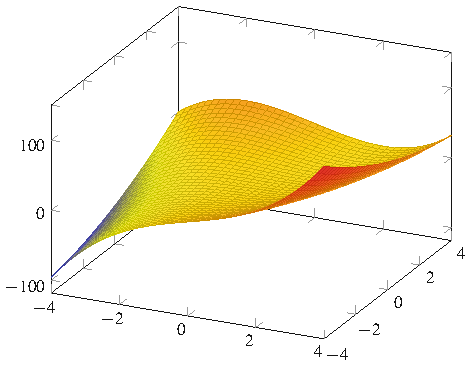
\includegraphics[width=0.559\linewidth]{images/vector/fig-2-4.pdf}
  \caption{函数 $f(x,y)=x^3+y^2-3xy$ 的图像}
  \label{fig:2-4}
\end{figure}

作为进一步的说明, 函数 $f(x,y)=xy$ 和 $f(x,y)=x^2+y^2$ 的图像如图 \ref{fig:2-5} 所示. 和之前一样, 实际作图所用的点集是 $\mathbb{R}^3$ 中的点 $(x,y,f(x,y))$, 因此可以看出, 画函数 $f:\mathbb{R}^2\to\mathbb{R}$ 的图像需要三个维度. 这意味着我们不能准确地画出任何函数 $f:\mathbb{R}^n\to\mathbb{R}$（$n\geq3$）的图像. 然而, 当我们想尝试可视化或描绘 $n\geq3$ 的函数 $f:\mathbb{R}^n\to\mathbb{R}$ 时, 我们常常继续画与图 \ref{fig:2-4} 和 \ref{fig:2-5} 类似的不准确的漫画.

\begin{figure}[htbp]
  \centering
  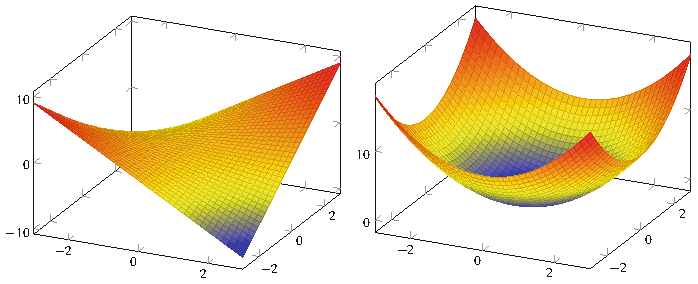
\includegraphics[width=0.960\linewidth]{images/vector/fig-2-5.pdf}
  \caption{作为二元函数图像示例的函数 $f(x,y)=xy$（左）与 $f(x,y)=x^2+y^2$（右）在 $\mathbb{R}^3$ 中的图像}
  \label{fig:2-5}
\end{figure}

我们将对流形 $\mathbb{R}^n$ 上的``函数''和向量空间 $\mathbb{R}^n$ 上的``函数''使用不同的名称. 流形 $\mathbb{R}^n$ 上的函数就简称为函数, 或者有时, 如果我们想强调值域是实数集, 就称为实值函数. 然而, 当值域是实数集时, 向量空间 $\mathbb{R}^n$ 上的``函数''称为泛函；当值域是另一个向量空间时, 称为变换. 我们已经花了一些时间考虑某一类泛函, 即满足
\[
f(v+w)=f(v)+f(w),\qquad f(cv)=cf(v)
\]
的线性泛函, 其中 $v$ 和 $w$ 是向量, $c$ 是实数. 所以, 流形 $\mathbb{R}^n$ 与向量空间 $\mathbb{R}^n$ 的区别隐含在我们的用语中：
\[
\text{函数 }f:\text{（流形）}\mathbb{R}^n\to\mathbb{R},\qquad
\text{泛函 }f:\text{（向量空间）}\mathbb{R}^n\to\mathbb{R}.
\]

现在, 我们将考虑一个从 $\mathbb{R}^n$ 到 $\mathbb{R}$ 的非常特殊的函数. 我们先用 $\mathbb{R}^2$ 作为例子. 我们要看的特殊函数称为坐标函数. 目前我们只看笛卡尔坐标函数.

考虑流形 $\mathbb{R}^2$ 中由笛卡尔坐标 $(3,5)$ 给出的点 $p$. 那么坐标函数
\[
x:\mathbb{R}^2\to\mathbb{R},\qquad p\longmapsto x(p)
\]
挑出第一个坐标, 即 $x(p)=x(3,5)=3$；坐标函数
\[
y:\mathbb{R}^2\to\mathbb{R},\qquad p\longmapsto y(p)
\]
挑出第二个坐标, $y(p)=y(3,5)=5$. 这在图 \ref{fig:2-6} 中作了说明.

\begin{figure}[htbp]
  \centering
  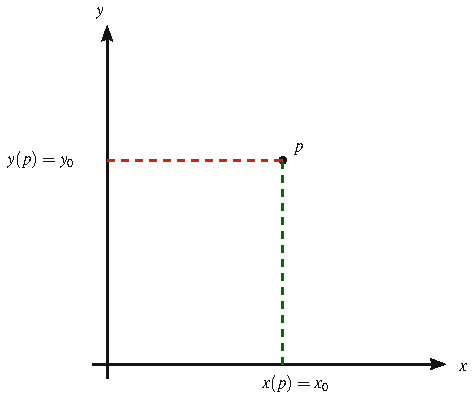
\includegraphics[width=0.562\linewidth]{images/vector/fig-2-6.pdf}
  \caption{坐标函数 $x:\mathbb{R}^2\to\mathbb{R}$ 与 $y:\mathbb{R}^2\to\mathbb{R}$ 分别挑出点 $p\in\mathbb{R}^2$ 的坐标值 $x_0$ 与 $y_0$}
  \label{fig:2-6}
\end{figure}

事实上, 尽管你习惯于把 $(3,5)$ 想成一个点, 但一个点实际上比这更抽象. 一个点独立于其坐标而存在. 例如, 你有时会看到这样的写法：
\[
p=\bigl(x(p),y(p)\bigr),
\]
例如, 对于我们上面给出的那个点, 有 $x(p)=3$, $y(p)=5$.

这里有一些我们需要习惯的歧义. 通常 $x$ 和 $y$ 被用来表示坐标函数 $x$ 和 $y$ 的输出值. 所以, 我们可能会遇到像下面这样有歧义的陈述
\[
x(p)=x,\qquad y(p)=y,
\]
其中等式左边的 $x$ 和 $y$ 是从 $\mathbb{R}^2$ 到 $\mathbb{R}$ 的坐标函数, 而右边的 $x$ 和 $y$ 是实数, 即 $\mathbb{R}$ 的元素. 学会识别 $x$ 和 $y$ 何时是坐标函数、何时是实数值, 需要一点练习, 你必须仔细观察它们是如何被使用的. 这种区别有时会被指出, 但常常被一带而过.

即使点是抽象的、独立于坐标的, 我们实际上也不能不给出一个``地址''就谈论一个特定的点. 这实际上正是坐标函数所做的, 它们被用来给点一个``地址''.

$\mathbb{R}^3$ 上（就此而言还有 $\mathbb{R}^n$ 上）的坐标函数是完全类似的. 例如, 在 $\mathbb{R}^3$ 上有三个坐标函数
\begin{align*}
x:\mathbb{R}^3\to\mathbb{R},\qquad y:\mathbb{R}^3\to\mathbb{R},\qquad z:\mathbb{R}^3\to\mathbb{R}, \\
p\longmapsto x(p),\qquad p\longmapsto y(p),\qquad p\longmapsto z(p),
\end{align*}
它们挑出点 $p$ 的 $x$、$y$、$z$ 坐标, 如图 \ref{fig:2-7} 所示.

\begin{figure}[htbp]
  \centering
  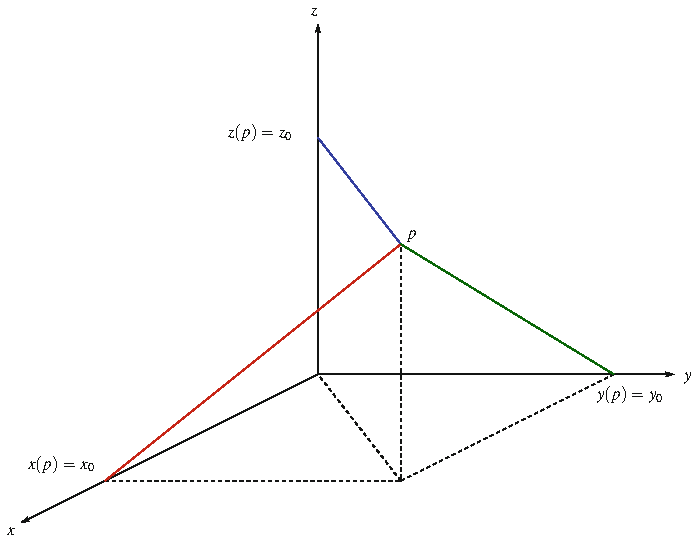
\includegraphics[width=0.827\linewidth]{images/vector/fig-2-7.pdf}
  \caption{坐标函数 $x:\mathbb{R}^3\to\mathbb{R}$、$y:\mathbb{R}^3\to\mathbb{R}$、$z:\mathbb{R}^3\to\mathbb{R}$ 分别挑出点 $p\in\mathbb{R}^3$ 的坐标值 $x_0,y_0,z_0$}
  \label{fig:2-7}
\end{figure}

当然, 笛卡尔坐标函数并不是仅有的坐标函数. 极坐标、球坐标和柱坐标函数是你可能遇到过的其他例子. 我们将在后面更详细地讨论这些坐标系, 但目前我们只考虑一个例子. 考虑点 $p=\bigl(x(p),y(p)\bigr)=(3,5)$. 极坐标 $r$ 和 $\theta$ 通常由 $x=r\cos(\theta)$ 和 $y=r\sin(\theta)$ 给出. 假设我们想求点 $p$ 用极坐标表示的``地址''. 也就是说, 我们想求 $p=\bigl(r(p),\theta(p)\bigr)$.
由于我们已知用 $x$ 和 $y$ 坐标表示的 $p$, 我们可以写 $r=\sqrt{x^2+y^2}$ 和 $\theta=\arctan\frac{y}{x}$. 于是我们有
\begin{align*}
p=\bigl(r(p),\theta(p)\bigr)
&=\Bigl(r\bigl(x(p),y(p)\bigr),\theta\bigl(x(p),y(p)\bigr)\Bigr)\\
&=\left(\sqrt{x(p)^2+y(p)^2},\;\arctan\frac{y(p)}{x(p)}\right)\\
&=\left(\sqrt{3^2+5^2},\;\arctan\frac{5}{3}\right)\\
&=\left(\underbrace{\sqrt{34}}_{r},\;\underbrace{\arctan\frac{5}{3}}_{\theta}\right)\\
&\approx(5.831,\;59.036).
\end{align*}
这里同样的歧义也适用, $r$ 和 $\theta$ 既可以是坐标函数, 也可以是坐标函数给出的值.

\section{切空间与向量场}

让我们回顾一下目前所做的工作. 我们已经回顾了向量空间, 并把 $\mathbb{R}^n$ 作为向量空间讨论, 即作为形如
\[
v=\begin{bmatrix}x_1\\\vdots\\x_n\end{bmatrix}
\]
（其中 $x_1,\ldots,x_n\in\mathbb{R}$）的向量的集合来讨论. 然后我们又把 $\mathbb{R}^n$ 作为流形讨论, 即作为点 $(x_1,\ldots,x_n)$（其中 $x_1,\ldots,x_n\in\mathbb{R}$）的集合来讨论. 我们还回顾了向量空间 $\mathbb{R}^n$ 上的线性泛函和流形 $\mathbb{R}^n$ 上的函数, 并引入了坐标函数. 现在我们来看看流形 $\mathbb{R}^n$ 如何与向量空间 $\mathbb{R}^n$ 相联系. 我们这样做的动机是做微积分的愿望. 嗯, 至少目前是为了取方向导数.

然而, 为了帮助我们更好地想象正在发生的事情, 我们将先考虑三个流形：$S^1$、$S^2$ 和 $T$. 流形 $S^1$ 就是一个圆, 流形 $S^2$ 是球面, 流形 $T$ 是环面, 看起来像一个甜甜圈. 目前我们将相当不精确. 我们希望你带走对流形是什么的一般感受, 而不是用技术细节压垮你. 目前我们只说流形是一个局部为欧几里得的空间. 我们的意思是, 如果我们观察流形的非常小的一部分, 那部分看起来就像某个自然数 $n$ 的 $\mathbb{R}^n$.

我们将对我们选择考察的三个流形说明这个思想. 圆 $S^1$ 局部像 $\mathbb{R}^1$, 这解释了 $S$ 上的上标 1. 在图 \ref{fig:2-8} 中, 我们几次放大 1-球面 $S^1$ 的一小部分, 以看出局部地流形 $S^1$ 看起来像 $\mathbb{R}^1$. 类似地, 在图 \ref{fig:2-9} 中我们放大 2-球面 $S^2$ 的一小部分, 以看出它局部像 $\mathbb{R}^2$；在图 \ref{fig:2-10} 中我们放大环面 $T$ 的一小部分, 以看出它局部也像 $\mathbb{R}^2$.

\begin{figure}[htbp]
  \centering
  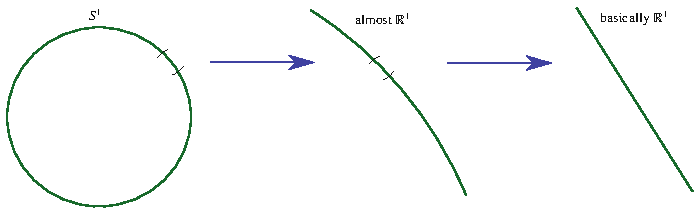
\includegraphics[width=0.944\linewidth]{images/vector/fig-2-8.pdf}
  \caption{这里放大了 1-球面（即圆）$S^1$ 的一小部分, 以显示局部地流形 $S^1$ 看起来像 $\mathbb{R}^1$}
  \label{fig:2-8}
\end{figure}

\begin{figure}[htbp]
  \centering
  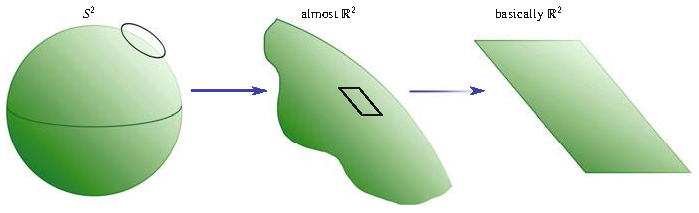
\includegraphics[width=0.953\linewidth]{images/vector/fig-2-9.pdf}
  \caption{这里放大了 2-球面 $S^2$ 的一小部分, 以显示局部地流形 $S^2$ 看起来像 $\mathbb{R}^2$}
  \label{fig:2-9}
\end{figure}

\begin{figure}[htbp]
  \centering
  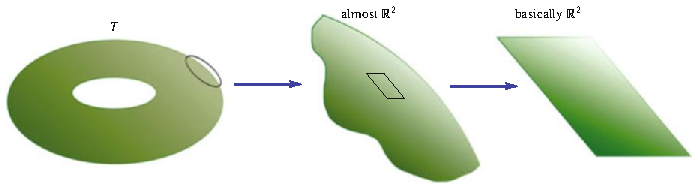
\includegraphics[width=0.960\linewidth]{images/vector/fig-2-10.pdf}
  \caption{这里放大了环面 $T$ 的一小部分, 以显示局部地流形 $T$ 看起来像 $\mathbb{R}^2$}
  \label{fig:2-10}
\end{figure}

这些例子的要点是, 即使这些示例流形局部看起来像 $\mathbb{R}^1$ 和 $\mathbb{R}^2$, 全局它们却并非如此. 也就是说, 它们的全局行为更为复杂；这些空间以欧几里得空间所没有的方式扭曲并重新连接自身.

现在我们引入切空间的概念. 同样, 我们想给你关于切空间是什么的一般感受, 而不是用技术细节压垮你, 这些将在 10.2 节给出. 从微积分中你应该记得曲线在其上某点处的切线是什么. 曲线的每个点都有它自己的切线, 如图 \ref{fig:2-11} 所示. 可以看出, 一维曲线的切空间是直线, 也就是说, 它们也是一维的.

类似地, 二维曲面在其每个点处都有一个切平面, 如图 \ref{fig:2-12} 所示. 流形在点 $p$ 处的切空间基本上是经过流形上点 $p$ 的光滑曲线在 $p$ 处的所有切线的集合. 这在图 \ref{fig:2-13} 中作了说明, 我们在那里画了一个点 $p$、五条经过它的光滑曲线, 以及这些曲线在点 $p$ 处的五条切线. 在这两幅图中切空间都是一个平面.

\begin{figure}[htbp]
  \centering
  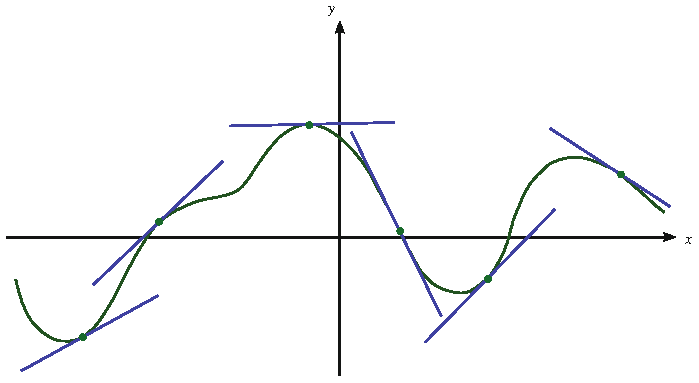
\includegraphics[width=0.838\linewidth]{images/vector/fig-2-11.pdf}
  \caption{这里画出一条曲线, 并在几个点处画出切线}
  \label{fig:2-11}
\end{figure}

\begin{figure}[htbp]
  \centering
  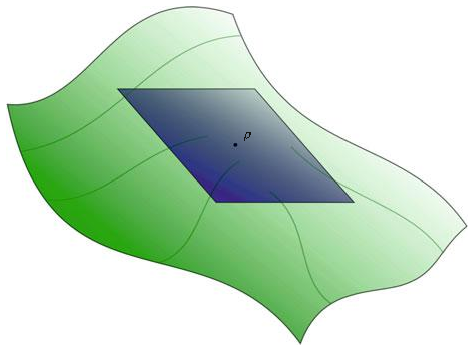
\includegraphics[width=0.610\linewidth]{images/vector/fig-2-12.pdf}
  \caption{这里画出一个二维曲面以及在一个点处画出的切平面}
  \label{fig:2-12}
\end{figure}

\begin{figure}[htbp]
  \centering
  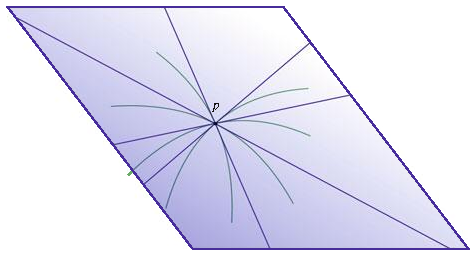
\includegraphics[width=0.662\linewidth]{images/vector/fig-2-13.pdf}
  \caption{二维曲面在点 $p$ 处的切平面是曲面上经过 $p$ 的曲线在 $p$ 处所有切线的集合}
  \label{fig:2-13}
\end{figure}

如果你想象三维流形中的一个点以及所有可能经过该点的曲线, 然后想象这些曲线在该点处的所有切线, 你就会看到该点处的切空间是三维的. 事实证明, 在``好''点处的切空间与该点处流形的维数相同. 在本书中我们不讨论在这个意义上不``好''的点处的流形. 事实上, 切空间无非就是正确 $n$ 值的向量空间 $\mathbb{R}^n$. 因为切空间是向量空间, 我们把点 $p$ 处的切空间想成点 $p$ 处所有切向量的集合. 我们使用切空间的特殊记号. $T_pM$ 或 $T_p(M)$ 表示流形 $M$ 在点 $p$ 处的切空间.

\begin{figure}[htbp]
  \centering
  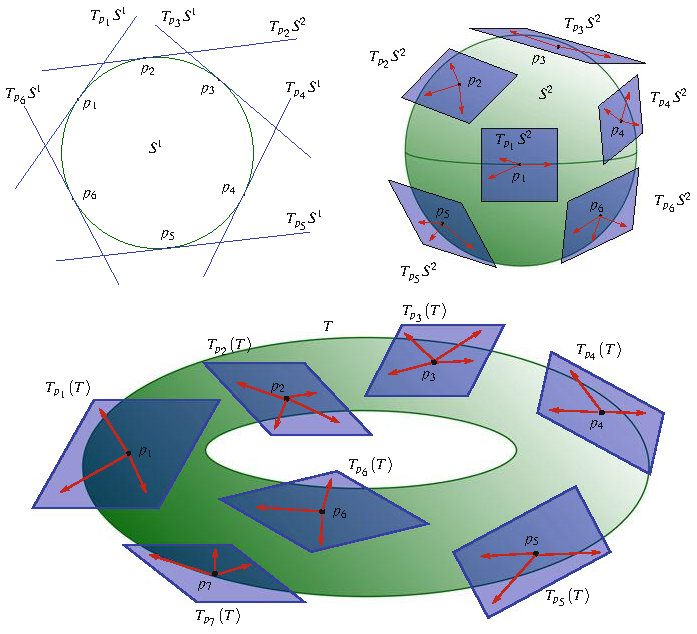
\includegraphics[width=0.826\linewidth]{images/vector/fig-2-14.pdf}
  \caption{流形 $S^1$ 以及若干画出的切线（左上）. 流形 $S^2$ 以及若干画出的切平面（右上）. 流形 $T$ 以及若干画出的切平面（下）. 对流形 $S^2$ 和 $T$, 还画出了每个切平面中的若干向量}
  \label{fig:2-14}
\end{figure}

为了更好了解流形的切空间集合长什么样, 我们在图 \ref{fig:2-14} 中为我们之前看过的三个简单流形画出了若干切空间：圆 $S^1$、球面 $S^2$ 和环面 $T$. 对二维切空间我们还画出了切空间的一些元素, 即从点 $p$ 出发的向量. 圆的切空间记为 $T_pS^1$, 球面的切空间记为 $T_pS^2$, 环面的切空间记为 $T_p(T)$. 这里使用圆括号只是因为 $T_pT$ 看起来有点奇怪.

尽管我们对流形 $\mathbb{R}^2$ 和 $\mathbb{R}^3$ 相当熟悉, 但想象这些流形的切空间有点奇怪, 尽管这正是你在向量微积分以来一直在隐式做的事情. 流形 $\mathbb{R}^2$ 在点 $p$ 处的切空间是基点在点 $p$ 的所有向量的集合. 在向量微积分中我们大量处理带不同基点的向量, 但我们总是把这些向量简单地想成在流形 $\mathbb{R}^2$ 或 $\mathbb{R}^3$ 中. 现在我们把这些向量想成属于附着在该点的一个单独的向量空间 $\mathbb{R}^2$ 或 $\mathbb{R}^3$ 的副本, 并称之为切空间.

\begin{figure}[htbp]
  \centering
  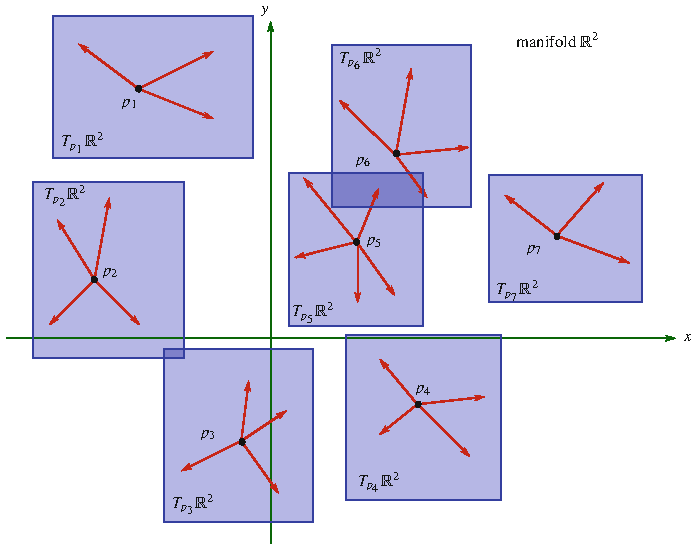
\includegraphics[width=0.960\linewidth]{images/vector/fig-2-15.pdf}
  \caption{流形 $\mathbb{R}^2$ 以及七个不同点处的切空间 $T_{p_i}\mathbb{R}^2$. 每个切空间中画出了若干向量}
  \label{fig:2-15}
\end{figure}

\begin{figure}[htbp]
  \centering
  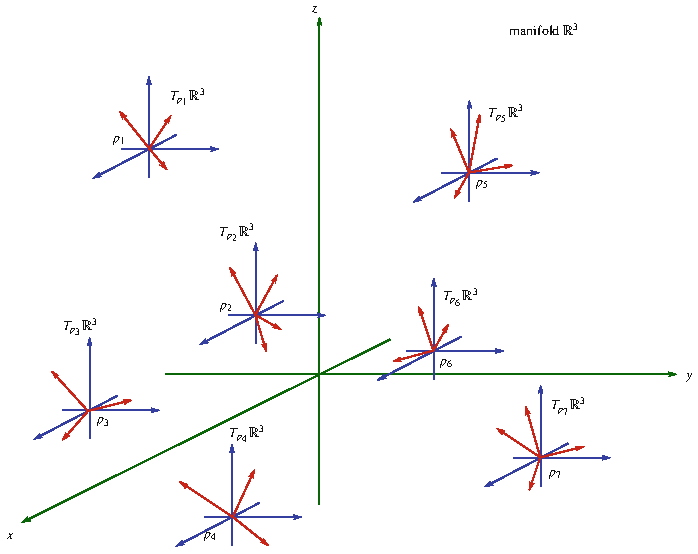
\includegraphics[width=0.960\linewidth]{images/vector/fig-2-16.pdf}
  \caption{流形 $\mathbb{R}^3$ 以及七个不同点处的切空间 $T_{p_i}\mathbb{R}^3$. 每个切空间中画出了若干向量}
  \label{fig:2-16}
\end{figure}

图 \ref{fig:2-15} 试图帮助你想象正在发生的事情. 图中画出了流形 $\mathbb{R}^2$ 以及七个不同点 $p_1,\ldots,p_7$ 处的切空间 $T_{p_i}\mathbb{R}^2$. 每个切空间 $T_p\mathbb{R}^2$ 都同构于（``等同于''）$\mathbb{R}^2$. 虽然我们只画出了七个点处的切空间, 但事实上对每个点 $p\in\mathbb{R}^2$ 都有一个单独的切空间 $T_p\mathbb{R}^2$.

图 \ref{fig:2-16} 试图帮助你想象 $\mathbb{R}^3$ 的切空间. 同样, 图中画出了流形 $\mathbb{R}^3$ 以及七个不同点 $p_1,\ldots,p_7$ 处的切空间 $T_{p_i}\mathbb{R}^3$. 每个切空间 $T_p\mathbb{R}^3$ 都自然同构于 $\mathbb{R}^3$. 同样, 虽然我们只画出了七个点处的切空间, 但事实上对每个点 $p\in\mathbb{R}^3$ 都有一个单独的切空间 $T_p\mathbb{R}^3$.

从现在起, 我们经常把向量的基点包含在记号中. 例如, 向量 $v_p$ 表示基点在流形 $M$ 的点 $p$ 处的向量 $v$. 显然, 向量 $v_p$ 属于（即是其中的元素）切空间 $T_pM$. 所以, 例如, 我们有
\[
\binom{1}{1}_{(-2,-3)}\in T_{(-2,-3)}\mathbb{R}^2,\qquad
\binom{1}{1}_{(-1,4)}\in T_{(-1,4)}\mathbb{R}^2,\qquad
\binom{1}{1}_{(2,4)}\in T_{(2,4)}\mathbb{R}^2,
\]
以及
\[
\begin{bmatrix}1\\1\\1\end{bmatrix}_{(-2,-3,-5)}\in T_{(-2,-3,-5)}\mathbb{R}^3,\qquad
\begin{bmatrix}1\\1\\1\end{bmatrix}_{(-1,4,3)}\in T_{(-1,4,3)}\mathbb{R}^3,\qquad
\begin{bmatrix}1\\1\\1\end{bmatrix}_{(2,4,-1)}\in T_{(2,4,-1)}\mathbb{R}^3.
\]

流形 $M$ 连同附着在流形每个点处的向量空间 $T_pM$ 的一个副本, 称为流形 $M$ 的切丛, 记为 $TM$ 或 $T(M)$. 流形 $M$ 的切丛的漫画版常常画成图 \ref{fig:2-17} 那样, 对流形和切空间都使用一维表示.

\begin{figure}[htbp]
  \centering
  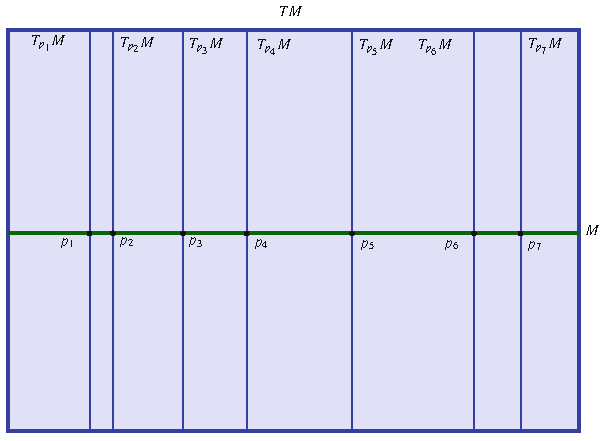
\includegraphics[width=0.749\linewidth]{images/vector/fig-2-17.pdf}
  \caption{流形 $M$ 上切丛 $TM$ 的漫画. 显示了七个切空间 $T_{p_i}M$}
  \label{fig:2-17}
\end{figure}

若 $M$ 是 $n$ 维流形, 则 $TM$ 是 $2n$ 维的. 这在直观上是合理的, 因为要精确指定 $TM$ 中任意元素（向量）, 你需要指定向量部分（需要 $n$ 个数）和基点（也需要 $n$ 个数）. 因此, $T\mathbb{R}^2$ 有四个维度, $T\mathbb{R}^3$ 有六个维度. 事实上, 流形 $M$ 的切丛 $TM$ 本身也是一个流形. 因此, 若 $M$ 是 $n$ 维流形, 则 $TM$ 是 $2n$ 维流形.

现在我们将非常简要地引入向量场的概念. 毫无疑问, 你在向量微积分中已经接触过向量场的思想, 在那里它通常定义在 $\mathbb{R}^2$ 或 $\mathbb{R}^3$ 上, 是一个给每个点 $(x,y)\in\mathbb{R}^2$ 或 $(x,y,z)\in\mathbb{R}^3$ 指派一个向量
\[
\binom{v_1}{v_2}_{(x,y)}\qquad\text{或}\qquad
\begin{bmatrix}v_1\\v_2\\v_3\end{bmatrix}_{(x,y,z)}
\]
的向量值函数. $\mathbb{R}^2$ 上的一个向量场示例如图 \ref{fig:2-18} 所示.

\begin{figure}[htbp]
  \centering
  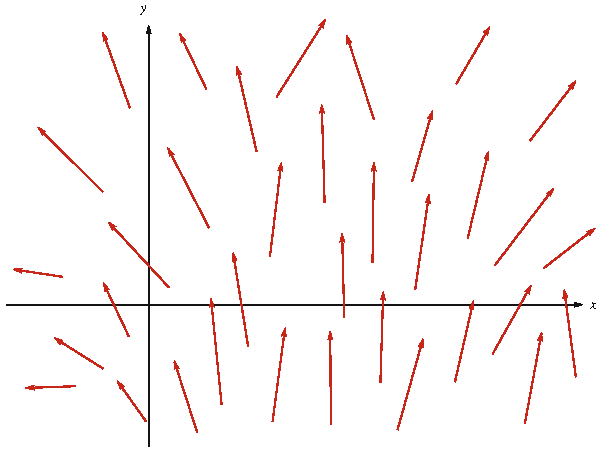
\includegraphics[width=0.756\linewidth]{images/vector/fig-2-18.pdf}
  \caption{画在流形 $\mathbb{R}^2$ 上的向量场. 回想一下, 所示的每个向量都是切空间的元素, 并不真正在流形 $\mathbb{R}^2$ 中}
  \label{fig:2-18}
\end{figure}

若可以在流形上找到一些曲线, 使得向量场中的所有向量都与这些曲线相切, 则称向量场是光滑的. 这些曲线称为向量场的积分曲线, 而求这些曲线本质上就是微分方程的全部内容. 图 \ref{fig:2-19} 显示了 $\mathbb{R}^2$ 上一个光滑向量场的若干积分曲线.

\begin{figure}[htbp]
  \centering
  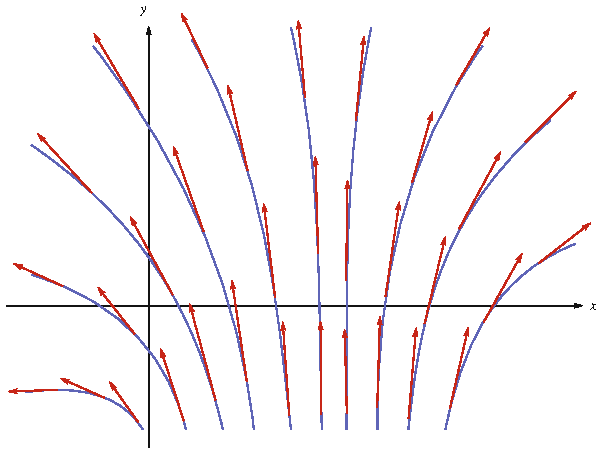
\includegraphics[width=0.756\linewidth]{images/vector/fig-2-19.pdf}
  \caption{画在流形 $\mathbb{R}^2$ 上的光滑向量场. 同样, 回想一下, 所示的每个向量都是切空间的元素, 并不真正在流形 $\mathbb{R}^2$ 中}
  \label{fig:2-19}
\end{figure}

虽然我们当然不打算在这里深入微分方程, 但我们想做的是引入一种思考向量场的新方式. 注意, 流形（如 $\mathbb{R}^2$ 或 $\mathbb{R}^3$）上的向量场在流形的每个点处给我们一个向量. 但流形 $M$ 的点 $p$ 处的向量 $v_p$ 是该点切空间 $T_pM$ 的元素. 所以, 给一个向量场与给 $M$ 的每个切空间的一个元素是同一回事. 这常被称为切丛 $TM$ 的一个截面. 在图形上, 我们常常像图 \ref{fig:2-20} 那样可视化切丛的截面.

\begin{figure}[htbp]
  \centering
  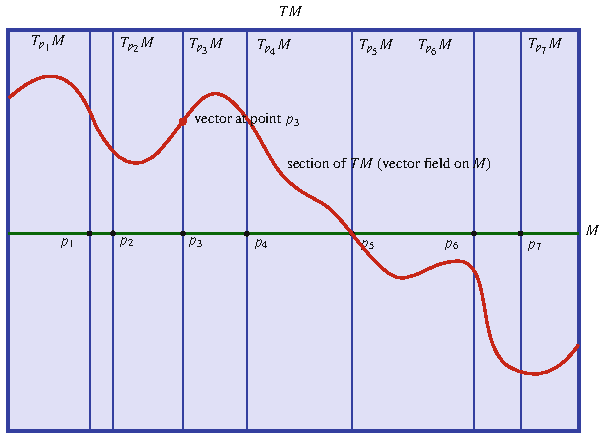
\includegraphics[width=0.749\linewidth]{images/vector/fig-2-20.pdf}
  \caption{流形 $M$ 上切丛的一个截面的漫画. $TM$ 的截面就是 $M$ 上的向量场. 向量场在 $M$ 的点 $p_3$ 处的向量被画成截面中 $T_{p_3}M$ 里的那个点. 注意, 在这种漫画表示中, 点 $p_5$ 处的向量将是零向量}
  \label{fig:2-20}
\end{figure}

\begin{question}\label{q:2-1}
在进入下一节之前, 让我们花一点时间回顾导数是怎么回事. 考虑由 $f(x)=\frac{x^2}{2}+2$ 给出的函数 $f:\mathbb{R}\to\mathbb{R}$.
\begin{enumerate}
  \item[(a)] 画出函数 $f(x)=\frac{x^2}{2}+2$ 的图像.
  \item[(b)] 求 $f(x)$ 的导数.
  \item[(c)] $f(2)$ 是什么？$f(3)$ 是什么？在点 $\bigl(2,f(2)\bigr)$ 和 $\bigl(3,f(3)\bigr)$ 之间画一条直线.
  \item[(d)] 这条割线的斜率是多少？
  \item[(e)] 写出差商定义导数的极限.
  \item[(f)] 用这个定义求 $f$ 在 $x=2$ 处的导数. 它与你上面得到的答案一致吗？
  \item[(g)] $f$ 在 $x=2$ 处的导数是一个数. 解释这个数代表什么.
\end{enumerate}
通过上面的问题, 你现在应该记得导数基本上就是函数图像在某点处切线的斜率.
\end{question}

\section{方向导数}

现在是时候探讨我们为什么要用这些材料了. 假设我们在流形 $\mathbb{R}^n$ 上有一个实值函数 $f$, 即 $f:\mathbb{R}^n\to\mathbb{R}$. 我们如何使用流形上某个给定点 $p$ 处的向量 $v_p$ 呢？一个自然的做法是取 $f$ 在点 $p$ 处沿 $v_p$ 方向的方向导数. 考虑图 \ref{fig:2-21}, 其中显示了实值函数 $f:\mathbb{R}\to\mathbb{R}$. 给定定义域中的一个点 $p$, 有两个可能移动的方向, 左或右. 类似地, 如果你有一个基点在该点的向量, 它既可以指向左（像 $v_p$ 那样）, 也可以指向右（像 $w_p$ 那样）. 我们可以问函数在这两个方向中的任一方向上如何变化. 在图 \ref{fig:2-22} 中描绘了实值函数 $f:\mathbb{R}^2\to\mathbb{R}$. 给定定义域中的一个点 $p=(x,y)$, 人们可以在二维中以任意方向移动, 而基点在该点的向量也可以在二维中指向任意方向. 类似地, 我们可以问函数在这些方向中的任意一个方向上如何变化. 在图 \ref{fig:2-23} 中我们选择了其中一个方向, 即由向量
\[
v_p=\binom{a}{b}_{(x,y)}
\]
给出的方向. 我们能利用这个向量求 $f$ 在点 $p$ 处沿 $v_p$ 方向的方向导数. 换句话说, 我们能求出 $f$ 在点 $p$ 处沿 $v_p$ 方向是如何变化的.

\begin{figure}[htbp]
  \centering
  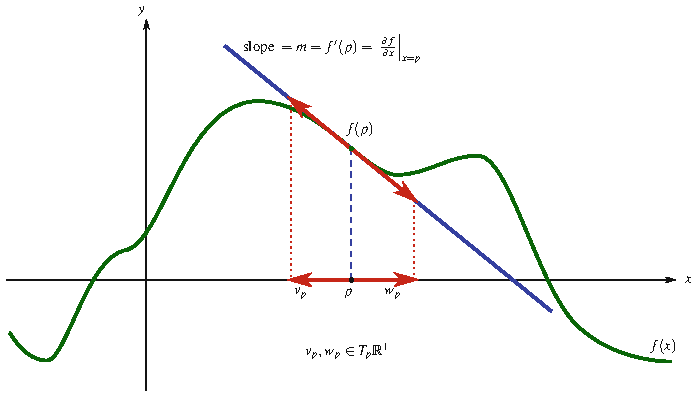
\includegraphics[width=0.877\linewidth]{images/vector/fig-2-21.pdf}
  \caption{从 $p\in\mathbb{R}$ 出发可以在任意一维方向上移动. 换句话说, 可以向右或向左}
  \label{fig:2-21}
\end{figure}

\begin{figure}[htbp]
  \centering
  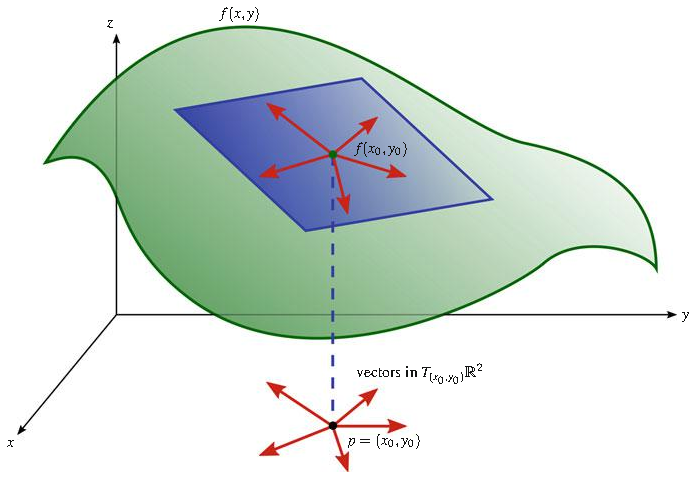
\includegraphics[width=0.829\linewidth]{images/vector/fig-2-22.pdf}
  \caption{从 $p=(x,y)\in\mathbb{R}^2$ 出发可以在二维中以任意方向移动. 图中画出了若干不同的方向}
  \label{fig:2-22}
\end{figure}

\begin{figure}[htbp]
  \centering
  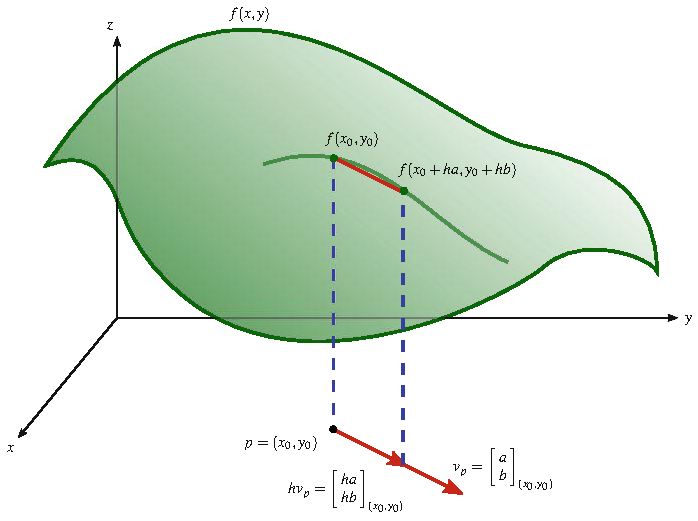
\includegraphics[width=0.834\linewidth]{images/vector/fig-2-23.pdf}
  \caption{求函数 $f:\mathbb{R}^2\to\mathbb{R}$ 的方向导数需要一个某个方向的单位向量以及 $f(x_0+ta,y_0+tb)$ 与 $f(x_0,y_0)$ 的相应值, 它们是差商所必需的}
  \label{fig:2-23}
\end{figure}

注意, 目前我们回到向量微积分的思考方式, 把向量 $v_p$ 想成位于流形 $\mathbb{R}^2$ 中的点 $p$ 处, 而不是在切空间 $T_p\mathbb{R}^2$ 中. 尽管我们刚刚大谈特谈向量不在流形中而在切空间中, 但由于在本节和下一节我们要从向量微积分的观点回顾方向导数的思想, 我们将回到把向量想成位于流形中、基点在某一点. 这样我们就能使用向量微积分的记号, 把注意力集中在相关的思想上, 而不被记号的细微差别拖累.

我们首先考虑方向导数在大多数多元微积分课程中通常是如何引入的. 我们这样做的原因是, 我们想使用的方向导数定义将与大多数向量微积分课程中使用的略有不同, 我们不希望有任何混淆. 你可能见过的定义是这样的.

\begin{definition}[方向导数（单位向量）]\label{def:2-3-1}
函数 $f:\mathbb{R}^2\to\mathbb{R}$ 在 $(x_0,y_0)$ 处沿单位向量 $u=\binom{a}{b}$ 方向的方向导数为
\[
D_uf(x_0,y_0)=\lim_{t\to0}\frac{f(x_0+ta,y_0+tb)-f(x_0,y_0)}{t},
\]
如果这个极限存在.
\end{definition}

\begin{definition}[方向导数（$\mathbb{R}^3$ 情形）]\label{def:2-3-2}
函数 $f:\mathbb{R}^3\to\mathbb{R}$ 在 $(x_0,y_0,z_0)$ 处沿单位向量 $u=\begin{bmatrix}a\\b\\c\end{bmatrix}$ 方向的方向导数为
\[
D_uf(x_0,y_0,z_0)=\lim_{t\to0}\frac{f(x_0+ta,y_0+tb,z_0+tc)-f(x_0,y_0,z_0)}{t},
\]
如果这个极限存在.
\end{definition}

通常向量微积分教科书会把向量写成行向量, 有时像 $[a,b]$, 有时像 $\langle a,b\rangle$. 我们在本书中绝不这样做. 我们总是把向量写成带方括号的列向量, $v=\binom{a}{b}$. 此外, 我们绝不使用尖括号 $\langle\cdot,\cdot\rangle$ 表示向量或点, 虽然有时会看到. 最后, 注意在两个定义中向量 $u$ 必须是单位向量, 这意味着向量的长度为一个单位. 换句话说, 对第一个定义我们必须有 $\sqrt{a^2+b^2}=1$, 对第二个定义我们必须有 $\sqrt{a^2+b^2+c^2}=1$.

为了提醒我们自己一些其他等价的记号, 注意如果我们令 $p=(x_0,y_0)$, 那么我们也可以写
\[
\lim_{t\to0}\frac{f(x_0+ta,y_0+tb)-f(x_0,y_0)}{t}
=\left.\frac{d}{dt}f(p+tu)\right|_{t=0}
\]
而如果我们令 $p=(x_0,y_0,z_0)$, 那么我们也可以写
\[
\lim_{t\to0}\frac{f(x_0+ta,y_0+tb,z_0+tc)-f(x_0,y_0,z_0)}{t}
=\left.\frac{d}{dt}f(p+tu)\right|_{t=0}.
\]
这意味着我们也可以把上面的定义写成
\[
D_uf(x_0,y_0)=\left.\frac{d}{dt}f(p+tu)\right|_{t=0}
\]
和
\[
D_uf(x_0,y_0,z_0)=\left.\frac{d}{dt}f(p+tu)\right|_{t=0}.
\]

假设我们有一个函数 $f:\mathbb{R}^2\to\mathbb{R}$ 和单位向量
\[
u=\binom{1}{0},\qquad v=\binom{0}{1},
\]
那么很容易看出 $D_uf=\frac{\partial f}{\partial x}$、$D_vf=\frac{\partial f}{\partial y}$. 类似地, 对函数 $g:\mathbb{R}^3\to\mathbb{R}$ 和单位向量
\[
u=\begin{bmatrix}1\\0\\0\end{bmatrix},\qquad v=\begin{bmatrix}0\\1\\0\end{bmatrix},\qquad w=\begin{bmatrix}0\\0\\1\end{bmatrix},
\]
我们得到 $D_ug=\frac{\partial g}{\partial x}$、$D_vg=\frac{\partial g}{\partial y}$、$D_wg=\frac{\partial g}{\partial z}$.

\begin{question}\label{q:2-2}
求 $f(x,y)=x^3-3xy+y^2$ 在 $p=(1,2)$ 处沿 $u=\binom{\cos(\pi/6)}{\sin(\pi/6)}$ 方向的导数.
\end{question}

按照你在多元微积分中可能做过的方式, 在做出上述方向导数定义之后, 推导出以下定理.

\begin{theorem}[方向导数的计算公式]\label{thm:2-1}
若 $f:\mathbb{R}^2\to\mathbb{R}$ 是关于 $x$ 和 $y$ 的可微函数, 则 $f$ 沿任意单位向量 $u=\binom{a}{b}$ 方向具有方向导数, 且
\[
D_uf(x,y)=\frac{\partial f}{\partial x}(x,y)\cdot a+\frac{\partial f}{\partial y}(x,y)\cdot b.
\]
\end{theorem}

\begin{proof}[证明梗概]
首先定义一元函数 $g(h)$ 为 $g(h)=f(x_0+ha,y_0+hb)$, 并用它改写 $D_uf$. 然后用链式法则写出 $g(h)$ 的导数. 最后令 $h=0$ 并合并.
\end{proof}

\begin{theorem}[方向导数的计算公式（$\mathbb{R}^3$ 情形）]\label{thm:2-2}
若 $f:\mathbb{R}^3\to\mathbb{R}$ 是关于 $x,y,z$ 的可微函数, 则 $f$ 沿任意单位向量 $u=\begin{bmatrix}a\\b\\c\end{bmatrix}$ 方向具有方向导数, 且
\[
D_uf(x,y,z)=\frac{\partial f}{\partial x}(x,y,z)\cdot a+\frac{\partial f}{\partial y}(x,y,z)\cdot b+\frac{\partial f}{\partial z}(x,y,z)\cdot c.
\]
\end{theorem}

\begin{question}\label{q:2-3}
令 $p=(2,0,-1)$, $v=\frac{1}{\sqrt{14}}\begin{bmatrix}2\\-1\\3\end{bmatrix}$. 求 $D_{v_p}f$, 其中
\begin{enumerate}
  \item[(a)] $f(x,y,z)=y^2z$
  \item[(b)] $f(x,y,z)=e^x\cos(y)$
  \item[(c)] $f(x,y,z)=x^7$
\end{enumerate}
\end{question}

现在我们想探讨为什么规定
\[
u=\binom{a}{b}\qquad\text{或}\qquad u=\begin{bmatrix}a\\b\\c\end{bmatrix}
\]
是单位向量. 我们首先注意到, 经过原点的平面方程由
\[
z=m_xx+m_yy
\]
给出, 如图 \ref{fig:2-24} 所示. 由此很容易证明, $f$ 图像上经过点 $(x_0,y_0,f(x_0,y_0))$ 的平面方程由
\[
z-f(x_0,y_0)=m_x(x-x_0)+m_y(y-y_0)
\]
给出.

\begin{figure}[htbp]
  \centering
  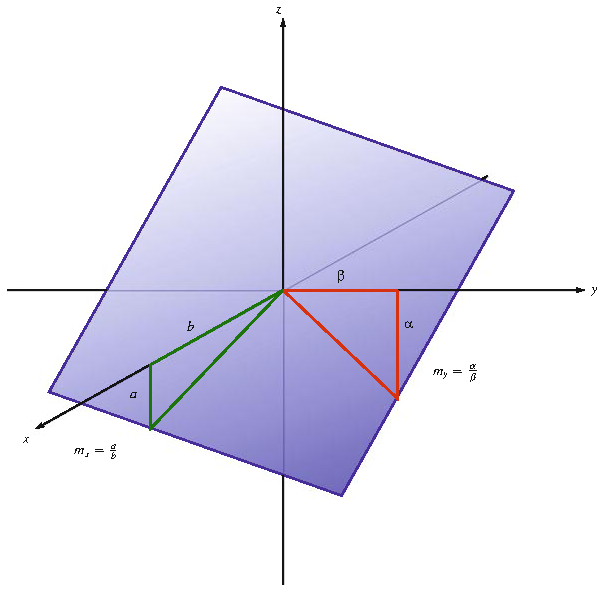
\includegraphics[width=0.777\linewidth]{images/vector/fig-2-24.pdf}
  \caption{经过原点的平面方程由 $z=m_xx+m_yy$ 给出, 其中 $m_x$ 是平面沿 $x$ 轴的斜率, $m_y$ 是平面沿 $y$ 轴的斜率}
  \label{fig:2-24}
\end{figure}

为得到 $f(x,y)$ 在点 $(x_0,y_0,f(x_0,y_0))$ 处切平面 $T(x_0,y_0)$ 的方程, 我们注意到
\begin{align*}
m_x=\frac{\partial f}{\partial x},\qquad m_y=\frac{\partial f}{\partial y} \\
\Rightarrow\quad T(x,y)-f(x_0,y_0)=\left.\frac{\partial f}{\partial x}\right|_{(x_0,y_0)}\cdot(x-x_0)+\left.\frac{\partial f}{\partial y}\right|_{(x_0,y_0)}\cdot(y-y_0), \\
\Rightarrow\quad T(x,y)=f(x_0,y_0)+\left.\frac{\partial f}{\partial x}\right|_{(x_0,y_0)}\cdot(x-x_0)+\left.\frac{\partial f}{\partial y}\right|_{(x_0,y_0)}\cdot(y-y_0),
\end{align*}
如图 \ref{fig:2-25} 所示.

\begin{figure}[htbp]
  \centering
  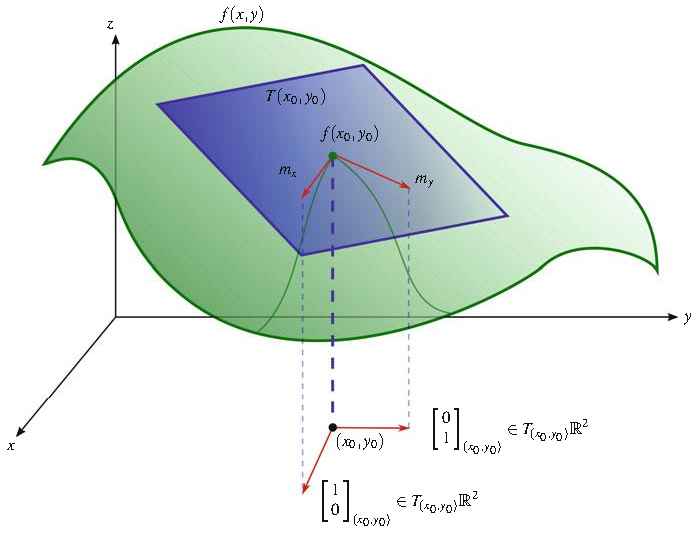
\includegraphics[width=0.891\linewidth]{images/vector/fig-2-25.pdf}
  \caption{$f(x,y)$ 在点 $(x_0,y_0,f(x_0,y_0))$ 处的切平面 $T(x_0,y_0)$}
  \label{fig:2-25}
\end{figure}

考虑点 $(x_0,y_0)$ 处的向量 $u=\binom{a}{b}$, 即 $u=\binom{a}{b}_{(x_0,y_0)}$, 如图 \ref{fig:2-26} 所示. 我们如何求经过点 $f(x_0,y_0)$ 的 $f$ 的图像切线的斜率呢？我们使用 $m=\frac{\text{rise}}{\text{run}}$, 其中显然``run''是向量 $\binom{a}{b}$ 的长度. 我们的 rise, 即高度 $z$ 的变化, 可以用我们上面推导的切平面方程计算, 
\begin{align*}
\frac{\text{rise}}{\text{run}}
&=\frac{T(x_0+a,y_0+b)-T(x_0,y_0)}{\sqrt{a^2+b^2}}\\
&=\frac{\left.\frac{\partial f}{\partial x}\right|_{(x_0,y_0)}\cdot a+\left.\frac{\partial f}{\partial y}\right|_{(x_0,y_0)}\cdot b}{\sqrt{a^2+b^2}}\\
&=\frac{\frac{\partial f}{\partial x}\cdot a+\frac{\partial f}{\partial y}\cdot b}{\sqrt{a^2+b^2}}.
\end{align*}

\begin{figure}[htbp]
  \centering
  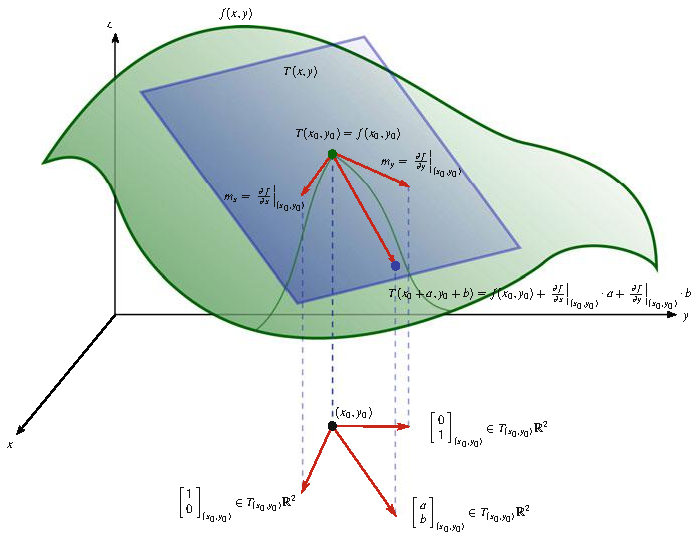
\includegraphics[width=0.960\linewidth]{images/vector/fig-2-26.pdf}
  \caption{$f(x,y)$ 在点 $(x_0,y_0)$ 处的切平面, 其中显示了沿方向 $v=ae_1+be_2$ 的切线}
  \label{fig:2-26}
\end{figure}

注意这与多元微积分中给出的 $D_uf$ 的公式多么接近：
\[
D_uf=\frac{\partial f}{\partial x}\cdot a+\frac{\partial f}{\partial y}\cdot b.
\]
只要向量 $\binom{a}{b}$ 是单位向量, 这两个公式就相同. 因此, 若 $u$ 是单位向量, 则 $D_uf$ 的公式也给出位于切平面内、沿 $\binom{a}{b}$ 方向的切线的斜率. 所以, 通过规定 $u=\binom{a}{b}$ 是单位向量, 我们基本上既保持了导数的定义是切线的斜率, 又保留了一个漂亮的简单导数公式.

我们现在将放宽这一要求, 允许任意向量, 而不只是单位向量. 然而, 我们想保留那个漂亮的公式. 这意味着我们需要放弃导数是切线斜率这一想法. 因此我们将与之前完全一样地定义方向导数, 但去掉 $u$ 必须是单位向量的规定. 为了得到切线的斜率, 我们将不得不把我们新的方向导数定义给出的值除以向量的长度. 那么, 我们新的方向导数定义实际上代表什么呢？它将代表上面方程中的``rise''部分——切线在向量 $u$ 的长度上有多少``rise''.

考虑图 \ref{fig:2-26}. 通过去掉 $u$ 是单位向量的要求, 方向导数
\[
D_uf=\frac{\partial f}{\partial x}\cdot a+\frac{\partial f}{\partial y}\cdot b
\]
告诉我们, 当我们沿着 $u$ 移动时, 函数 $f$ 的图像在点 $(x_0,y_0)$ 处的切平面``上升''了多少. 因此方向导数实际上告诉我们函数在该点处的切平面的某些信息. 我们还花一点时间指出, 函数 $f$ 在点 $(x_0,y_0)$ 处的切平面实际上是函数 $f$ 的图像在 $(x_0,y_0)$ 处最接近的线性逼近.

现在花一点时间考虑我们对方向导数在多元微积分课程中通常引入方式的回顾. 从头到尾都没有提到流形 $\mathbb{R}^2$ 或 $\mathbb{R}^3$ 的切空间. 在多元微积分中人们可以而且确实把切空间与底层流形混为一谈或合并在一起, 因为它们本质上是同一个空间. 然而, 最终当我们开始处理其他类型的流形时, 我们将不能再这样做. 这就是为什么我们如此努力地始终做出这一区别.

\begin{definition}[方向导数（任意向量）]\label{def:2-3-3}
设 $f:\mathbb{R}^n\to\mathbb{R}$ 是流形 $\mathbb{R}^n$ 上的实值函数, $v_p$ 是与流形 $\mathbb{R}^n$ 相切的向量, 即 $v_p\in T_p(\mathbb{R}^n)$. 数
\[
v_p[f]\equiv\left.\frac{d}{dt}f(p+tv_p)\right|_{t=0}
\]
称为 $f$ 关于 $v_p$ 的方向导数, 如果它存在.
\end{definition}

这与多元微积分情形中的定义完全相同, 只是去掉了 $v_p$ 必须是单位向量的要求. 因此, 如果 $v_p$ 不是单位向量, 我们从这个方向导数定义得到的数将不是切线的斜率, 而是当我们移动 $v_p$ 的长度时 $f$ 的图像在点 $p$ 处切线的``rise''.

还要注意新记号 $v_p[f]$. 这个记号与函数记号 $f(x)$ 非常相似, 函数 $f$``吃进''一个输入值 $x$ 并给出一个数. 在记号 $v_p[f]$ 中, 向量 $v_p$``吃进''一个函数 $f$ 并给出一个数：$f$ 在方向 $v_p$（在点 $p$ 处）的方向导数. 所以, 向量 $v_p$ 变成了所谓的函数 $f$ 上的算子. 基本上, 算子是把其他函数作为输入的函数.

\begin{question}\label{q:2-4}
令 $v=\begin{bmatrix}2\\-1\\3\end{bmatrix}$, $p=(2,0,-1)$.
\begin{enumerate}
  \item[(a)] 求 $v_p[f]$, 其中
  \begin{enumerate}
    \item[(i)] $f(x)=x$, 
    \item[(ii)] $f(x)=x^2-x$, 
    \item[(iii)] $f(x)=\cos(x)$.
  \end{enumerate}
  \item[(b)] 对上面每个函数, 求 $w_p[f]$, 其中
  \begin{enumerate}
    \item[(i)] $w_p=2v_p$, 
    \item[(ii)] $w_p=\frac12v_p$, 
    \item[(iii)] $w_p=-5v_p$, 
    \item[(iv)] $w_p=-\frac15v_p$.
  \end{enumerate}
\end{enumerate}
\end{question}

假设我们有一个函数 $f:\mathbb{R}^3\to\mathbb{R}$ 和点 $p=(p_1,p_2,p_3)$ 处的向量 $v_p=\begin{bmatrix}v_1\\v_2\\v_3\end{bmatrix}_p\in T_p(\mathbb{R}^3)$, 我们想求 $v_p[f]$ 的表达式. 首先把 $p+tv_p$ 写为 $p+tv_p=(p_1+tv_1,p_2+tv_2,p_3+tv_3)$, 于是
\[
f(p+tv_p)=f(p_1+tv_1,p_2+tv_2,p_3+tv_3).
\]
其次我们注意到, 若对 $i=1,2,3$ 定义函数 $x_i(t)=p_i+tv_i$, 则有 $\frac{dx_i}{dt}=\frac{d}{dt}(p_i+tv_i)=v_i$. 把这一切放在一起并使用链式法则, 我们发现
\begin{align*}
v_p[f]&=\left.\frac{d}{dt}f(p+tv)\right|_{t=0}\\
&=\left.\frac{d}{dt}f(p_1+tv_1,p_2+tv_2,p_3+tv_3)\right|_{t=0}\\
&\qquad\underbrace{\qquad\quad}_{x_1(t)}\quad\underbrace{\qquad\quad}_{x_2(t)}\quad\underbrace{\qquad\quad}_{x_3(t)}\\
&=\left.\frac{\partial f}{\partial x_1}\right|_{x_1(0)}\cdot\left.\frac{dx_1}{dt}\right|_{t=0}
+\left.\frac{\partial f}{\partial x_2}\right|_{x_2(0)}\cdot\left.\frac{dx_2}{dt}\right|_{t=0}
+\left.\frac{\partial f}{\partial x_3}\right|_{x_3(0)}\cdot\left.\frac{dx_3}{dt}\right|_{t=0}\\
&=\left.\frac{\partial f}{\partial x_1}\right|_{p_1}\cdot v_1+\left.\frac{\partial f}{\partial x_2}\right|_{p_2}\cdot v_2+\left.\frac{\partial f}{\partial x_3}\right|_{p_3}\cdot v_3\\
&=\sum_{i=1}^{3}v_i\cdot\left.\frac{\partial f}{\partial x_i}\right|_{p}
\end{align*}
总之, 在这个例子中我们刚刚发现
\[
v_p[f]=\sum_{i=1}^{3}v_i\cdot\left.\frac{\partial f}{\partial x_i}\right|_{p}.
\]

特别地, 假设我们有一个流形 $\mathbb{R}^3$ 上的实值函数 $f:\mathbb{R}^3\to\mathbb{R}$, 以及标准欧几里得向量
\[
e_1=\begin{bmatrix}1\\0\\0\end{bmatrix},\qquad e_2=\begin{bmatrix}0\\1\\0\end{bmatrix},\qquad e_3=\begin{bmatrix}0\\0\\1\end{bmatrix}.
\]
暂时我们从记号中略去基点, 因为它不起什么特别的作用. 由于 $v[f]=\sum_{i=1}^{3}v_i\cdot\frac{\partial f}{\partial x_i}$, 我们有 $e_1[f]=\frac{\partial f}{\partial x_1}$、$e_2[f]=\frac{\partial f}{\partial x_2}$、$e_3[f]=\frac{\partial f}{\partial x_3}$. 我们实际上刚刚证明了非常有趣的事情. 通过非常轻微的记号改变, 它变得更加明显
\[
e_1[f]=\frac{\partial}{\partial x_1}f,\qquad e_2[f]=\frac{\partial}{\partial x_2}f,\qquad e_3[f]=\frac{\partial}{\partial x_3}f.
\]
我们刚刚把算子 $\frac{\partial}{\partial x_i}$ 与欧几里得向量 $e_i$ 等同起来. 在短短一段里, 我们证明了本书中最重要的思想之一.

\begin{center}
\fbox{\parbox{0.86\textwidth}{\centering
欧几里得向量 $e_i$ 可以与偏微分算子 $\dfrac{\partial}{\partial x_i}$ 等同
}}
\end{center}

换句话说, 我们可以把欧几里得向量 $e_i$ 想成实际上就是偏微分算子 $\frac{\partial}{\partial x_i}$.

\begin{question}\label{q:2-5}
重做上面的计算并把基点 $p$ 放进记号中, 以使你自己确信基点 $p$ 在计算中不起任何作用.
\end{question}

\begin{question}\label{q:2-6}
设 $a,b\in\mathbb{R}$, $p$ 是流形 $\mathbb{R}^3$ 上的一个点, $v_p,w_p\in T_p(\mathbb{R}^3)$, $f,g:\mathbb{R}^3\to\mathbb{R}$.
\begin{enumerate}
  \item[(a)] 证明 $(av_p+bw_p)[f]=av_p[f]+bw_p[f]$.
  \item[(b)] 证明 $v_p[af+bg]=av_p[f]+bv_p[g]$.
\end{enumerate}
\end{question}

除了上面问题中成立的恒等式之外, 还有一条称为 Leibnitz 法则的性质成立. Leibnitz 法则说的是 $v_p[fg]=v_p[f]\cdot g(p)+f(p)\cdot v_p[g]$. 本质上 Leibnitz 法则就是乘积法则, 它实际上被用于证明这一恒等式, 
\begin{align*}
v_p[fg]&=\sum_{i=1}^{3}v_i\cdot\left.\frac{\partial fg}{\partial x_i}\right|_{p_i}\\
&=\sum_{i=1}^{3}v_i\cdot\left(\left.\frac{\partial f}{\partial x_i}\right|_{p}\cdot g(p)+f(p)\cdot\left.\frac{\partial g}{\partial x_i}\right|_{p}\right)\\
&=\left(\sum_{i=1}^{3}v_i\left.\frac{\partial f}{\partial x_i}\right|_{p}\right)g(p)+f(p)\left(\sum_{i=1}^{3}v_i\left.\frac{\partial g}{\partial x_i}\right|_{p}\right)\\
&=v_p[f]\cdot g(p)+f(p)\cdot v_p[g].
\end{align*}

首先, 我们花一点时间指出一个记号上的歧义. 当我们给出一个向量 $v$ 时, 通常用下标表示向量所在的基点, 所以 $v_p$ 意味着向量 $v$ 的基点在点 $p$. 但这里, 对欧几里得单位向量 $e_1,e_2,e_3$, 下标显然不是指一个点, 它指的是哪个笛卡尔坐标非零（事实上是等于 $1$）. 欧几里得单位向量非常常见而记号非常有用, 我们通常在用到它们时省略基点 $p$. 当然人们可以写 $e_{1_p}$、$e_{2_p}$、$e_{3_p}$, 但过一会儿这就变得有点傻了. 通常从上下文应该能清楚基点到底是什么.

既然做了这个小记号说明, 我们就可以沉浸在我们刚刚完成的光辉成就中, 同时试图消化它. 最近这几页（以上一个例子达到高潮）实际上比表面看起来深刻得多, 所以我们将花一点时间重申刚刚完成了什么.

首先, 你以前见过向量, 可能对它们相当熟悉, 至少在 $n$ 维欧几里得空间中的向量是如此. 当然, 现在我们把这些向量看成切空间的元素, 但它们仍然只是老式的向量. 其次, 你以前见过微分, 可能对微分算子很熟悉, 像 $\frac{d}{dx}$、$\frac{d}{dt}$、$\frac{\partial}{\partial x}$、$\frac{\partial}{\partial y}$, 尽管你也有可能没见过把算子一词用在它们身上.

给定函数 $f:\mathbb{R}^3\to\mathbb{R}$, 我们利用取 $f$ 在点 $p\in\mathbb{R}^3$ 处沿 $v_p\in T_p\mathbb{R}^3$ 方向的方向导数这一行为, 把向量 $v_p\in T_p\mathbb{R}^3$ 变成了 $f$ 上的算子. 这给出了下面的公式
\[
v_p[f]=\sum_{i=1}^{3}v_i\cdot\left.\frac{\partial f}{\partial x_i}\right|_{p_i}.
\]
这个公式随后被用来确切地看欧几里得单位向量 $e_1,e_2,e_3$ 在点 $p$ 处的算子是什么, 我们确定可以做以下等同：
\[
e_1\equiv\frac{\partial}{\partial x_1},\qquad
e_2\equiv\frac{\partial}{\partial x_2},\qquad
e_3\equiv\frac{\partial}{\partial x_3}.
\]
如果你以前没见过, 这真的是一个令人惊讶的等同. 它无疑感觉有点像记号的障眼法. 但这是恰到好处的记号的力量之一, 它帮助你理解那些可能难以以其他方式把握的关系. 通过把切空间中的向量看成通过方向导数作用在函数上, 我们把向量与偏微分算子等同起来. 见图 \ref{fig:2-27}. 这是我们在本书其余部分将继续做出的等同.

\begin{figure}[htbp]
  \centering
  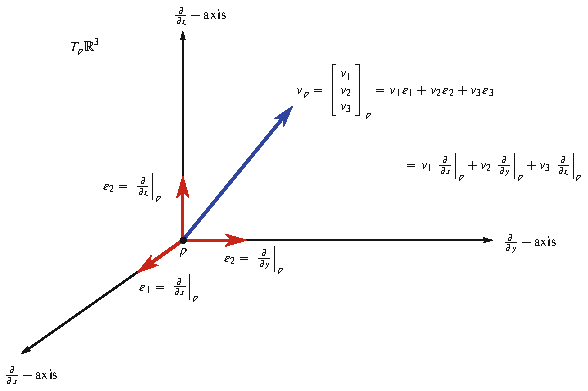
\includegraphics[width=0.960\linewidth]{images/vector/fig-2-27.pdf}
  \caption{把欧几里得向量 $e_i$ 与偏微分算子 $\partial/\partial x_i$ 等同}
  \label{fig:2-27}
\end{figure}

把这个等同付诸实践, 考虑向量
\[
v=\begin{bmatrix}2\\-3\\1\end{bmatrix}.
\]
当用欧几里得单位向量 $e_1,e_2,e_3$ 写 $v$ 时, 我们有
\[
v=2e_1-3e_2+e_3,
\]
而当用微分算子写它时, 我们有
\[
v=2\frac{\partial}{\partial x_1}-3\frac{\partial}{\partial x_2}+\frac{\partial}{\partial x_3}.
\]

从现在起我们将对 $e_1,e_2,e_3$ 与 $\frac{\partial}{\partial x_1},\frac{\partial}{\partial x_2},\frac{\partial}{\partial x_3}$ 之间作很少或不作区别, 视情况使用任何一种记号. 你还应该注意, 你可能经常看到 $\frac{\partial}{\partial x_1},\frac{\partial}{\partial x_2},\frac{\partial}{\partial x_3}$ 写为 $\partial_1,\partial_2,\partial_3$, 或 $\partial_{x_1},\partial_{x_2},\partial_{x_3}$, 甚至 $\partial_x,\partial_y,\partial_z$. 如果我们想考虑基点, 比如说
\[
v_p=\begin{bmatrix}v_1\\v_2\\v_3\end{bmatrix}_p\in T_p(\mathbb{R}^3),
\]
那么我们会写
\[
v_p=v_1\left.\frac{\partial}{\partial x_1}\right|_{p}+v_2\left.\frac{\partial}{\partial x_2}\right|_{p}+v_3\left.\frac{\partial}{\partial x_3}\right|_{p}.
\]

\section{微分 1-形式}

让我们回顾一下我们所做的. 首先我们回顾了向量空间与对偶空间. 之后我们区分了流形（流形 $\mathbb{R}^3$）与向量空间（向量空间 $\mathbb{R}^3$）, 并引入了切空间 $T_p(\mathbb{R}^3)$ 的概念, 它基本上是附着在流形 $\mathbb{R}^3$ 每个点 $p$ 上的一个向量空间 $\mathbb{R}^3$. 之后我们回顾了方向导数, 并用它们发现了向量与偏微分算子之间的一个恒等关系. 我们发现每个向量 $v_p\in T_p(\mathbb{R}^3)$ 恰好是一个微分算子
\[
v_p=\begin{bmatrix}v_1\\v_2\\v_3\end{bmatrix}_p=v_1\left.\frac{\partial}{\partial x_1}\right|_{p}+v_2\left.\frac{\partial}{\partial x_2}\right|_{p}+v_3\left.\frac{\partial}{\partial x_3}\right|_{p}.
\]
认识到每个切空间 $T_p(\mathbb{R}^n)$ 本身是一个向量空间, 显然每个切空间 $T_p(\mathbb{R}^n)$ 都有自己的对偶空间, 记为 $T_p^*(\mathbb{R}^n)$. 我们现在要看的正是这个空间.

我们现在已经准备好迎接我们一直等待的定义, 微分 1-形式的定义.

\begin{definition}[微分 1-形式]\label{def:2-4-1}
流形 $\mathbb{R}^n$ 上的微分 1-形式 $\alpha$ 是流形 $\mathbb{R}^n$ 的切向量集合上的线性泛函. 也就是说, 在流形 $\mathbb{R}^n$ 的每个点 $p$ 处, $\alpha:T_p(\mathbb{R}^n)\to\mathbb{R}$, 并且
\[
\alpha(v_p+w_p)=\alpha(v_p)+\alpha(w_p),\qquad \alpha(av_p)=a\alpha(v_p)
\]
对所有 $v_p,w_p\in T_p(\mathbb{R}^n)$ 和 $a\in\mathbb{R}$ 成立.
\end{definition}

需要做一些评注来帮助你更好地理解这个定义. 首先, 我们在讨论向量空间时已经定义了线性泛函. 向量空间所有线性泛函的集合称为该向量空间的对偶空间. 在 1-形式的定义中, 向量空间是 $T_p(\mathbb{R}^n)$. $T_p(\mathbb{R}^n)$ 的对偶空间通常记为 $T_p^*(\mathbb{R}^n)$. 因此, 我们有 $\alpha\in T_p^*(\mathbb{R}^n)$.

接下来要注意的是, 在定义中第一个所需恒等式的左边, 加法发生在向量空间 $T_p(\mathbb{R}^n)$ 中. 换句话说, $v_p+w_p\in T_p(\mathbb{R}^n)$. 等号右边的加法发生在实数集 $\mathbb{R}$ 中. 也就是说, $\alpha(v_p)+\alpha(w_p)\in\mathbb{R}$. 术语上还有一个小的怪癖：$\alpha$ 被称为流形 $\mathbb{R}^n$ 上的微分 1-形式, 尽管它的输入是向量, 即流形 $\mathbb{R}^n$ 中某个点 $p$ 处流形切空间 $T_p(\mathbb{R}^n)$ 的元素. 所以, 即使 $\alpha$ 吃进的是流形 $\mathbb{R}^n$ 的切空间 $T_p(\mathbb{R}^n)$ 的元素, 它仍被称为流形 $\mathbb{R}^n$ 上的微分 1-形式. 如果我们想指明微分形式所在的点, 我们将使用 $\alpha_p$ 或 $\alpha(p)$. 显然我们有 $\alpha_p\in T_p^*(\mathbb{R}^n)$, 即 $T_p(\mathbb{R}^n)$ 的对偶空间.

那么, 为什么叫微分 1-形式呢？加上的``1-''是因为它只把一个切向量作为输入. 后面我们将遇到 2-形式、3-形式和一般的 $k$-形式, 它们分别把两个、三个或 $k$ 个切向量作为输入. ``微分''一词是因为形式与外微分思想之间的密切关系, 我们将在后面研究. 最后, ``形式''一词是一个有点通用的数学术语, 被用于相当广泛的一类对象（双线性形式、二次形式、多重线性形式、第一和第二基本形式等等）. 因此, 微分 $k$-形式是一个数学对象, 其输入是某点处的 $k$ 个向量, 并且与某种关于微分的想法有关. 很多时候``微分''一词被省去, 微分 $k$-形式被简称为 $k$-形式. 到目前为止这个定义还有点抽象, 因此为了更好地理解, 我们现在将考虑流形 $\mathbb{R}^3$ 上一些具体而简单的 1-形式例子. 但在我们写出流形 $\mathbb{R}^3$ 上 1-形式的具体例子之前, 我们需要决定 $T_p^*(\mathbb{R}^3)$ 的一组基.

基于我们对向量空间的回顾以及那里使用的记号, 对偶基写成向量空间基的上标形式而不是下标形式. 假设我们把 $T_p(\mathbb{R}^3)$ 的基写成 $\{e_{1_p},e_{2_p},e_{3_p}\}$, 那么我们也许可以尝试把 $T_p^*(\mathbb{R}^3)$ 的基写成 $\{e_p^1,e_p^2,e_p^3\}$. 但回想标准欧几里得单位向量与微分算子之间的等同, 我们也可以把 $T_p(\mathbb{R}^3)$ 的基写成
\[
\left\{\left.\frac{\partial}{\partial x_1}\right|_{p},\left.\frac{\partial}{\partial x_2}\right|_{p},\left.\frac{\partial}{\partial x_3}\right|_{p}\right\}.
\]
但现在我们怎么写对偶基呢？我们把对偶基, 即对偶空间 $T_p^*(\mathbb{R}^3)$ 的基, 写为
\[
\{dx_{1_p},dx_{2_p},dx_{3_p}\}.
\]
是的, 这组基看起来像你在微积分中熟悉的微分. 这是有原因的. 一旦我们做了几道题, 你对这个记号更熟悉一点之后, 我们将探讨这个记号的原因. 从记号中略去基点 $p$, 我们将写
\[
\{dx_1,dx_2,dx_3\}
\]
作为与 $T(\mathbb{R}^3)$ 的基
\[
\left\{\frac{\partial}{\partial x_1},\frac{\partial}{\partial x_2},\frac{\partial}{\partial x_3}\right\}
\]
对偶的 $T^*(\mathbb{R}^3)$ 的基. 图 \ref{fig:2-28} 试图以图形方式画出流形 $\mathbb{R}^3$、点 $p$ 处的切空间 $T_p\mathbb{R}^3$ 及其对偶空间 $T_p^*\mathbb{R}^3$. 我们常常认为切空间 $T_p\mathbb{R}^3$ 和对偶空间 $T_p^*(\mathbb{R}^3)$``附着''在流形 $\mathbb{R}^3$ 的点 $p$ 上, 但我们在图中把对偶空间 $T_p^*\mathbb{R}^3$ 画在切空间 $T_p\mathbb{R}^3$ 的正上方. 对偶空间 $T_p^*\mathbb{R}^3$ 通常称为 $p$ 处的余切空间.

\begin{figure}[htbp]
  \centering
  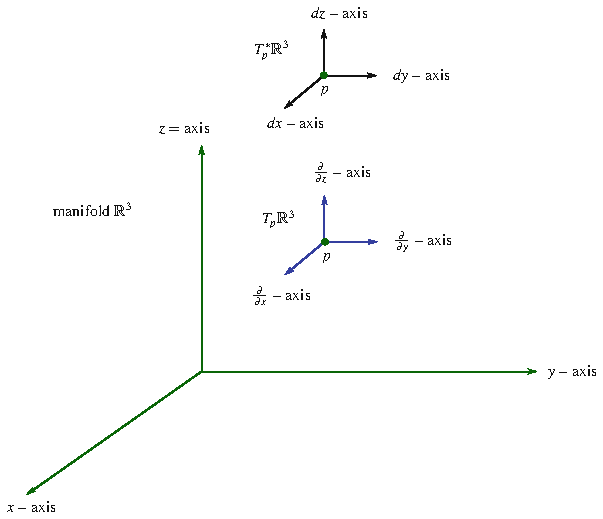
\includegraphics[width=0.715\linewidth]{images/vector/fig-2-28.pdf}
  \caption{流形 $\mathbb{R}^3$ 以及``附着''在点 $p$ 处的切空间 $T_p\mathbb{R}^3$ 的图示. 对偶空间 $T_p^*\mathbb{R}^3$ 画在它所对偶的切空间上方. 注意轴标记方式的不同}
  \label{fig:2-28}
\end{figure}

由于 $T_p^*\mathbb{R}^3$ 的任意元素都可以写成 $\{dx_1,dx_2,dx_3\}$ 的线性组合, 而 $T_p^*\mathbb{R}^3$ 的元素是 1-形式, 这当然意味着 $\mathbb{R}^3$ 上的 1-形式可以写成 $\{dx_1,dx_2,dx_3\}$ 的线性组合. 特别地, 基元素 $dx_1,dx_2,dx_3$ 本身是 $\mathbb{R}^3$ 上的 1-形式.

现在我们将确切地看到对偶基, 即 1-形式 $\{dx_1,dx_2,dx_3\}$, 如何作用于切空间基元素 $\frac{\partial}{\partial x_1},\frac{\partial}{\partial x_2},\frac{\partial}{\partial x_3}$. 由对偶基的定义, 我们有
\begin{align*}
dx_1\left(\frac{\partial}{\partial x_1}\right)=1,\qquad dx_2\left(\frac{\partial}{\partial x_1}\right)=0,\qquad dx_3\left(\frac{\partial}{\partial x_1}\right)=0, \\
dx_1\left(\frac{\partial}{\partial x_2}\right)=0,\qquad dx_2\left(\frac{\partial}{\partial x_2}\right)=1,\qquad dx_3\left(\frac{\partial}{\partial x_2}\right)=0, \\
dx_1\left(\frac{\partial}{\partial x_3}\right)=0,\qquad dx_2\left(\frac{\partial}{\partial x_3}\right)=0,\qquad dx_3\left(\frac{\partial}{\partial x_3}\right)=1.
\end{align*}

现在让我们考虑一个向量, 比如说
\[
\begin{bmatrix}-1\\3\\-4\end{bmatrix}=-\frac{\partial}{\partial x_1}+3\frac{\partial}{\partial x_2}-4\frac{\partial}{\partial x_3},
\]
看看微分形式 $dx_1,dx_2,dx_3$ 如何作用于它. 首先看 $dx_1$ 如何作用于这个向量：
\begin{align*}
dx_1\left(-\frac{\partial}{\partial x_1}+3\frac{\partial}{\partial x_2}-4\frac{\partial}{\partial x_3}\right)
&=dx_1\left(-\frac{\partial}{\partial x_1}\right)+dx_1\left(3\frac{\partial}{\partial x_2}\right)+dx_1\left(-4\frac{\partial}{\partial x_3}\right)\\
&=-dx_1\left(\frac{\partial}{\partial x_1}\right)+3dx_1\left(\frac{\partial}{\partial x_2}\right)-4dx_1\left(\frac{\partial}{\partial x_3}\right)\\
&=-1(1)+3(0)-4(0)\\
&=-1.
\end{align*}
类似地, 我们有
\begin{align*}
dx_2\left(-\frac{\partial}{\partial x_1}+3\frac{\partial}{\partial x_2}-4\frac{\partial}{\partial x_3}\right)
&=-dx_2\left(\frac{\partial}{\partial x_1}\right)+3dx_2\left(\frac{\partial}{\partial x_2}\right)-4dx_2\left(\frac{\partial}{\partial x_3}\right)\\
&=-1(0)+3(1)-4(0)\\
&=3
\end{align*}
以及
\begin{align*}
dx_3\left(-\frac{\partial}{\partial x_1}+3\frac{\partial}{\partial x_2}-4\frac{\partial}{\partial x_3}\right)
&=-dx_3\left(\frac{\partial}{\partial x_1}\right)+3dx_3\left(\frac{\partial}{\partial x_2}\right)-4dx_3\left(\frac{\partial}{\partial x_3}\right)\\
&=-1(0)+3(0)-4(1)\\
&=-4.
\end{align*}
本质上, 微分 1-形式 $dx_1,dx_2,dx_3$ 求出向量在相应轴上的投影. 回到更传统的 $x,y,z$ 记号, 1-形式 $dx$ 求出 $v_p$ 在 $\frac{\partial}{\partial x}$ 轴上的投影, 1-形式 $dy$ 求出 $v_p$ 在 $\frac{\partial}{\partial y}$ 轴上的投影, 1-形式 $dz$ 求出 $v_p$ 在 $\frac{\partial}{\partial z}$ 轴上的投影. 这在图 \ref{fig:2-29} 中作了图示.

\begin{figure}[htbp]
  \centering
  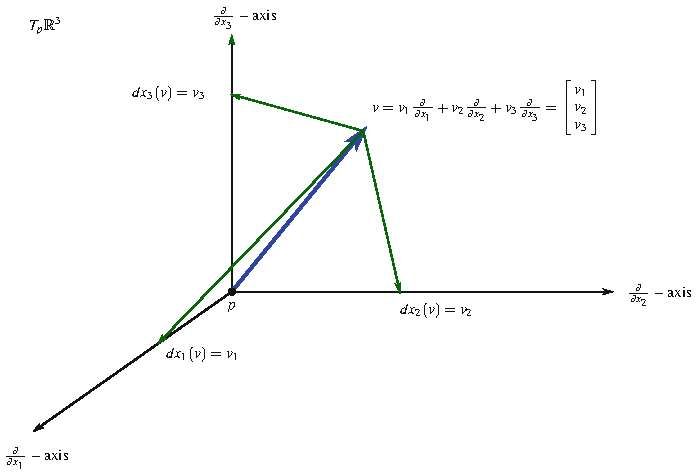
\includegraphics[width=0.845\linewidth]{images/vector/fig-2-29.pdf}
  \caption{对偶基元素如何作用于向量 $v$ 的图示. 该图在记号中没有包含点 $p$}
  \label{fig:2-29}
\end{figure}

\begin{question}\label{q:2-7}
求下列各值：
\begin{enumerate}
  \item[(a)] $dx_1\left(2\frac{\partial}{\partial x_1}+3\frac{\partial}{\partial x_1}\right)$
  \item[(b)] $dx_2\left(-\frac{\partial}{\partial x_1}+3\frac{\partial}{\partial x_2}-4\frac{\partial}{\partial x_3}\right)$
  \item[(c)] $dx_3\left(7\frac{\partial}{\partial x_2}-5\frac{\partial}{\partial x_3}\right)$
\end{enumerate}
\end{question}

由于集合 $\{dx,dy,dz\}$ 是 $T_p^*\mathbb{R}^3$ 的基, 任意元素 $\alpha\in T_p^*\mathbb{R}^3$ 都可以写成 $adx+bdy+cdz$ 的形式, 其中 $a,b,c\in\mathbb{R}$. 这些 1-形式的行为完全如你所预期. 例如, 考虑 1-形式 $2dx-3dy+5dz$ 如何作用于向量 $-\frac{\partial}{\partial x_1}+3\frac{\partial}{\partial x_2}-4\frac{\partial}{\partial x_3}$：
\begin{align*}
(2dx-3dy+5dz)\left(-\frac{\partial}{\partial x}+3\frac{\partial}{\partial y}-4\frac{\partial}{\partial z}\right)
&=2dx\left(-\frac{\partial}{\partial x}+3\frac{\partial}{\partial y}-4\frac{\partial}{\partial z}\right)\\
&\quad-3dy\left(-\frac{\partial}{\partial x}+3\frac{\partial}{\partial y}-4\frac{\partial}{\partial z}\right)\\
&\quad+5dz\left(-\frac{\partial}{\partial x}+3\frac{\partial}{\partial y}-4\frac{\partial}{\partial z}\right)\\
&=(2)(-1)(1)+(2)(3)(0)+(2)(-4)(0)\\
&\quad+(-3)(-1)(0)+(-3)(3)(1)+(-3)(-4)(0)\\
&\quad+(5)(-1)(0)+(5)(3)(0)+(5)(-4)(1)\\
&=-31.
\end{align*}
我们格外小心地展示了这个计算的每一步, 这是我们在未来当然不会总是做的.

\begin{question}\label{q:2-8}
求下列各值：
\begin{enumerate}
  \item[(a)] $(dx_1+dx_2)\left(5\frac{\partial}{\partial x_1}\right)$
  \item[(b)] $(2dx_2-3dx_3)\left(3\frac{\partial}{\partial x_1}-7\frac{\partial}{\partial x_2}+5\frac{\partial}{\partial x_3}\right)$
  \item[(c)] $(-dx_1-4dx_2+6dx_3)\left(-2\frac{\partial}{\partial x_1}+5\frac{\partial}{\partial x_2}-3\frac{\partial}{\partial x_3}\right)$
\end{enumerate}
\end{question}

为了使计算更简单, 1-形式常常写成行向量, 正如我们在向量空间的回顾中把对偶空间的元素写成行向量一样. 例如, 1-形式 $4dx_1-2dx_2+5dx_3$ 可以写成行向量 $[4,-2,5]$. 回想我们说过 $p$ 处的对偶空间常称为 $p$ 处的余切空间. 因此, 当一个 1-形式（余切空间的元素）写成行向量时, 它常被称为余向量. 这使得我们可以把上面的计算当作矩阵乘法来做. 让我们重做最后一个计算看看怎么做, 
\begin{align*}
(2dx-3dy+5dz)\left(-\frac{\partial}{\partial x}+3\frac{\partial}{\partial y}-4\frac{\partial}{\partial z}\right)
&=[2,-3,5]\begin{bmatrix}-1\\3\\-4\end{bmatrix}\\
&=(2)(-1)+(-3)(3)+(5)(-4)\\
&=-31.
\end{align*}
这当然是一个更直接的计算.

\begin{question}\label{q:2-9}
先把 1-形式写成行向量（余向量）、把向量元素写成列向量, 然后作为矩阵乘法做下列计算.
\begin{enumerate}
  \item[(a)] $(-7dx_1+dx_2)\left(2\frac{\partial}{\partial x_2}\right)$
  \item[(b)] $dx_3\left(7\frac{\partial}{\partial x_2}-5\frac{\partial}{\partial x_3}\right)$
  \item[(c)] $(2dx_2-3dx_3)\left(3\frac{\partial}{\partial x_1}-7\frac{\partial}{\partial x_2}+5\frac{\partial}{\partial x_3}\right)$
  \item[(d)] $(-dx_1-4dx_2+6dx_3)\left(-2\frac{\partial}{\partial x_1}+5\frac{\partial}{\partial x_2}-3\frac{\partial}{\partial x_3}\right)$
\end{enumerate}
\end{question}

注意我们现在有两种不同的心智图像可以用来尝试描绘微分 1-形式. 考虑图 \ref{fig:2-30}. 上面是作为行向量的微分 1-形式的图像, 这是最容易有的图像. 形如 $adx+bdy+cdz$（$a,b,c\in\mathbb{R}$）的微分 1-形式是某点处余切空间 $T_p^*\mathbb{R}^3$ 的元素, 所以把它们想象成行向量（称为余向量）是很自然的. 第二种图像是把 1-形式 $dx,dy,dz$ 看作求向量 $v_p$ 在不同轴上投影的方式. 在这种情况下, 1-形式 $adx+bdy+cdz$ 可以被看作分别按因子 $a,b,c$ 缩放相应的投影, 然后把这些不同的缩放加起来.

\begin{figure}[htbp]
  \centering
  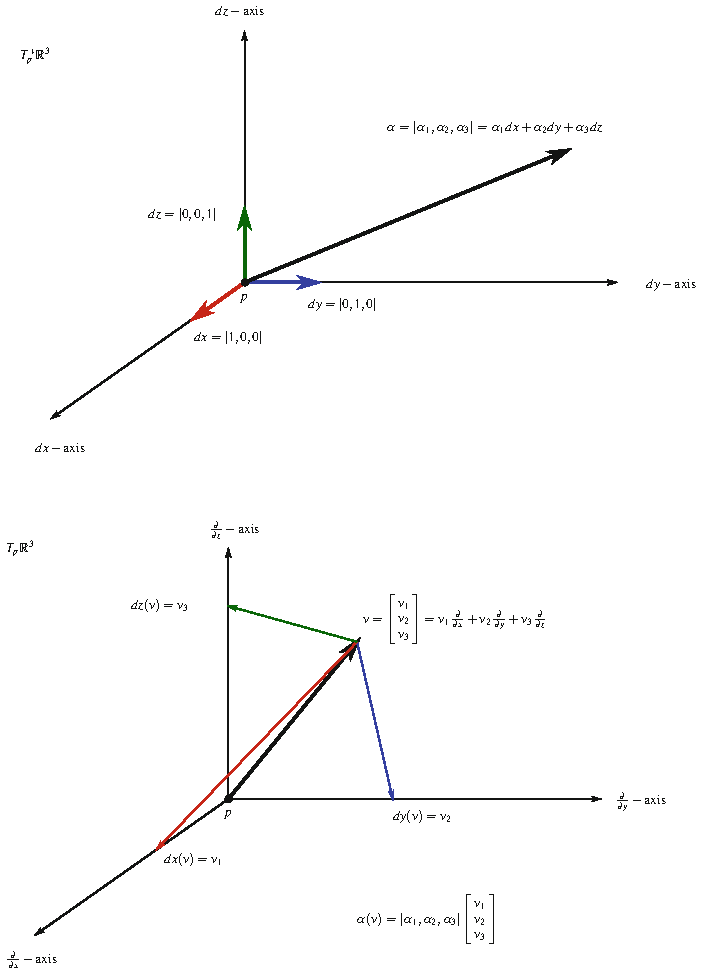
\includegraphics[width=0.896\linewidth]{images/vector/fig-2-30.pdf}
  \caption{想象或可视化微分 1-形式的两种不同方式. 作为 $T_p^*\mathbb{R}^3$ 中的余向量（上）, 或作为 $T_p\mathbb{R}^3$ 中向轴投影的线性组合（下）}
  \label{fig:2-30}
\end{figure}

在最后几道题中我们隐式地假设 1-形式和向量都在流形的同一点. 但正如向量给了我们向量场, 我们可以想象流形 $\mathbb{R}^3$ 上的 1-形式``场''. 然而实际上, 我们一般不会称它们为场, 我们只简称为 1-形式. 还记得那个有点奇怪的术语``流形 $\mathbb{R}^3$ 上的 1-形式''吗？流形上的 1-形式实际上是一个 1-形式场, 它在流形的每个点 $p$ 处给出一个特定的 1-形式, 作用于基点在该点的切向量 $v_p$.

让我们考虑一个例子. 给定流形 $\mathbb{R}^3$ 上的下列实值函数：$f(x,y,z)=x^2y$、$g(x,y,z)=\frac{x^2}{2}+yz$ 和 $h(x,y,z)=x+y+3$. 在流形 $\mathbb{R}^3$ 的每个点 $p=(x,y,z)$ 处, 通过
\[
\varphi_{(x,y,z)}=f(x,y,z)dx+g(x,y,z)dy+h(x,y,z)dz
\]
定义流形 $\mathbb{R}^3$ 上的 1-形式 $\varphi$. 流形 $\mathbb{R}^3$ 上的 1-形式 $\varphi$ 在 $\mathbb{R}^3$ 的每个点 $p$ 处定义一个不同的 1-形式. 例如, 在点 $(1,2,3)$ 处, 1-形式 $\varphi_{(1,2,3)}$ 由
\[
\varphi_{(1,2,3)}=f(1,2,3)dx+g(1,2,3)dy+h(1,2,3)dz=2dx+\frac{13}{2}dy+6dz
\]
给出. 如果我们给定向量
\[
v_p=\begin{bmatrix}2\\-1\\-2\end{bmatrix}_p
\]
在 $p=(1,2,3)$ 处, 我们将有
\begin{align*}
\varphi_p(v_p)&=\left(2dx+\frac{13}{2}dy+6dz\right)\left(2\frac{\partial}{\partial x}-1\frac{\partial}{\partial y}-2\frac{\partial}{\partial z}\right)\\
&=\left[2,\frac{13}{2},6\right]_{(1,2,3)}\begin{bmatrix}2\\-1\\-2\end{bmatrix}_{(1,2,3)}\\
&=2(2)+\frac{13}{2}(-1)+6(-2)\\
&=\frac{-29}{2}.
\end{align*}

因此, 给定流形 $\mathbb{R}^3$ 上的一个 1-形式 $\varphi$, 在 $\mathbb{R}^3$ 的每个点 $p$ 处我们都有一个映射 $\varphi_p:T_p(\mathbb{R}^3)\to\mathbb{R}$. 如果给定流形 $\mathbb{R}^3$ 上的一个向量场 $v$, 即切丛 $T\mathbb{R}^3$ 的一个截面, 那么对每个 $p\in\mathbb{R}^3$ 都有 $\varphi_p(v_p)\in\mathbb{R}$. 那么 $\varphi(v)$ 会是什么呢？注意我们没有放入一个点. 我们可以把 $\varphi(v)$ 考虑为流形 $\mathbb{R}^3$ 上的一个函数. 也就是说, 它的输入是流形上的点 $p$, 输出是实数, 像这样
\[
\varphi(v):\mathbb{R}^3\to\mathbb{R},\qquad p\longmapsto\varphi_p(v_p).
\]

\begin{question}\label{q:2-10}
对 1-形式 $\varphi_{(x,y,z)}=f(x,y,z)dx+g(x,y,z)dy+h(x,y,z)dz$, 其中 $f(x,y,z)=xy^2$、$g(x,y,z)=\frac{x^2}{3}+x$、$h(x,y,z)=xy+yz+xz$, 以及向量
\[
v_p=\begin{bmatrix}x\\x^2y\\xz\end{bmatrix}_p,
\]
求：
\begin{enumerate}
  \item[(a)] (i) $\varphi_{(-1,2,1)}$, (ii) $\varphi_{(0,-1,2)}$, (iii) $\varphi_{(8,4,-3)}$.
  \item[(b)] 求 $\varphi(v)$.
  \item[(c)] (i) 对 $p=(-1,2,1)$ 求 $\varphi_p(v_p)$；(ii) 对 $p=(0,-1,2)$ 求 $\varphi_p(v_p)$；(iii) 对 $p=(8,4,-3)$ 求 $\varphi_p(v_p)$.
\end{enumerate}
\end{question}

既然我们对 1-形式实际上做什么更熟悉了一些, 我们就准备好尝试更好地理解这个记号了. 本质上, 我们要理解我们把 $dx,dy,dz$ 记为与 $T_p(\mathbb{R}^3)$ 的基 $\frac{\partial}{\partial x},\frac{\partial}{\partial y},\frac{\partial}{\partial z}$ 对偶的 $T_p^*(\mathbb{R}^3)$ 的基的理由. 首先我们再做另一个定义, 乍一看它可能对你显得有点循环.

\begin{definition}[函数的微分]\label{def:2-4-2}
设 $f:\mathbb{R}^n\to\mathbb{R}$ 是流形 $\mathbb{R}^n$ 上的函数. $f$ 的微分 $df$ 被定义为 $\mathbb{R}^n$ 上满足如下条件的 1-形式：对所有向量 $v_p$, 
\[
df(v_p)=v_p[f].
\]
\end{definition}

让我们花一点时间考虑流形 $\mathbb{R}^3$, 试着解开并消化这一切. 首先, 给定流形 $\mathbb{R}^3$ 上的函数 $f:\mathbb{R}^3\to\mathbb{R}$ 和流形 $\mathbb{R}^3$ 中点 $p$ 处的向量 $v_p\in T_p(\mathbb{R}^3)$, 我们知道如何取这个函数在点 $p$ 处沿方向 $v_p$ 的方向导数
\[
\lim_{t\to0}\frac{f(p+tv_p)-f(p)}{t},
\]
它也可以写成
\[
\left.\frac{d}{dt}f(p+tv_p)\right|_{t=0}.
\]
然后我们认为这是用向量 $v_p$ 对给定函数 $f$ 施行一个运算, 于是为此引入了一个稍微新的记号
\[
v_p[f]=\left.\frac{d}{dt}f(p+tv_p)\right|_{t=0},
\]
反过来我们刚刚又用它定义了 $f$ 的微分, 写为 $df$, 由 $df(v_p)=v_p[f]$ 给出. 令 $p=(x_0,y_0,z_0)$, 我们把这一切放在一起得到
\begin{align*}
df(v_p)&=v_p[f]\\
&=\left.\frac{d}{dt}f(p+tv_p)\right|_{t=0}\\
&=\left.\frac{d}{dt}f(x_0+tv_1,y_0+tv_2,z_0+tv_3)\right|_{t=0}\\
&\qquad\underbrace{\qquad\qquad}_{x(t)}\quad\underbrace{\qquad\qquad}_{y(t)}\quad\underbrace{\qquad\qquad}_{z(t)}\\
&=\left.\frac{\partial f}{\partial x}\right|_{p}\cdot\left.\frac{dx(t)}{dt}\right|_{t=0}
+\left.\frac{\partial f}{\partial y}\right|_{p}\cdot\left.\frac{dy(t)}{dt}\right|_{t=0}
+\left.\frac{\partial f}{\partial z}\right|_{p}\cdot\left.\frac{dz(t)}{dt}\right|_{t=0}\\
&=\left.\frac{\partial f}{\partial x}\right|_{p}\cdot v_1+\left.\frac{\partial f}{\partial y}\right|_{p}\cdot v_2+\left.\frac{\partial f}{\partial z}\right|_{p}\cdot v_3.
\end{align*}
总之我们有
\[
df(v_p)=\left.\frac{\partial f}{\partial x}\right|_{p}\cdot v_1+\left.\frac{\partial f}{\partial y}\right|_{p}\cdot v_2+\left.\frac{\partial f}{\partial z}\right|_{p}\cdot v_3.
\]

由于这个公式对任意函数 $f:\mathbb{R}^3\to\mathbb{R}$ 都成立, 它对特殊的笛卡尔坐标函数 $x,y,z:\mathbb{R}^3\to\mathbb{R}$ 也成立. 回想笛卡尔坐标函数：若 $p\in\mathbb{R}^3$, 则 $x(p)$ 是 $p$ 的笛卡尔 $x$ 坐标值, $y(p)$ 是 $p$ 的笛卡尔 $y$ 坐标值, $z(p)$ 是 $p$ 的笛卡尔 $z$ 坐标值. 例如, 如果我们能用笛卡尔坐标把点 $p$ 写为 $(3,2,1)$, 那么 $x(p)=3$、$y(p)=2$、$z(p)=1$. 现在让我们确切地看看这些笛卡尔坐标函数每一个会发生什么. 假设
\[
v_p=\begin{bmatrix}v_1\\v_2\\v_3\end{bmatrix}_p=v_1\left.\frac{\partial}{\partial x}\right|_{p}+v_2\left.\frac{\partial}{\partial y}\right|_{p}+v_3\left.\frac{\partial}{\partial z}\right|_{p}.
\]
那么对笛卡尔坐标函数 $x:\mathbb{R}^3\to\mathbb{R}$, 我们有
\begin{align*}
dx(v_p)&=\left.\frac{\partial x}{\partial x}\right|_{p}\cdot v_1+\left.\frac{\partial x}{\partial y}\right|_{p}\cdot v_2+\left.\frac{\partial x}{\partial z}\right|_{p}\cdot v_3\\
&=(1)\cdot v_1+(0)\cdot v_2+(0)\cdot v_3\\
&=v_1.
\end{align*}
但当我们写 $\frac{\partial x}{\partial x}$ 时是什么意思呢？分子中的 $x$ 是笛卡尔坐标函数, 而分母中的 $x$ 表示我们对其求导的变量. 因此 $\frac{\partial x}{\partial x}$ 给出笛卡尔坐标函数 $x$ 在 $x$ 方向的变化率.

\begin{question}\label{q:2-11}
解释笛卡尔坐标函数 $x$ 在 $x$ 方向的变化率确实是一, 从而证明 $\frac{\partial x}{\partial x}=1$. 考虑当点 $p$ 在 $x$ 方向移动时 $x(p)$ 如何变化, 可能会有所帮助. 笛卡尔坐标函数 $x$ 在 $y$ 和 $z$ 方向的变化率是多少？解释你的答案如何证明 $\frac{\partial x}{\partial y}=0$ 和 $\frac{\partial x}{\partial z}=0$.
\end{question}

类似地, 我们有
\begin{align*}
dy(v_p)&=\left.\frac{\partial y}{\partial x}\right|_{p}\cdot v_1+\left.\frac{\partial y}{\partial y}\right|_{p}\cdot v_2+\left.\frac{\partial y}{\partial z}\right|_{p}\cdot v_3\\
&=(0)\cdot v_1+(1)\cdot v_2+(0)\cdot v_3\\
&=v_2
\end{align*}
以及
\begin{align*}
dz(v_p)&=\left.\frac{\partial z}{\partial x}\right|_{p}\cdot v_1+\left.\frac{\partial z}{\partial y}\right|_{p}\cdot v_2+\left.\frac{\partial z}{\partial z}\right|_{p}\cdot v_3\\
&=(0)\cdot v_1+(0)\cdot v_2+(1)\cdot v_3\\
&=v_3.
\end{align*}

\begin{question}\label{q:2-12}
求笛卡尔坐标函数 $y$ 在 $x,y,z$ 方向的变化率, 并用它证明 $\frac{\partial y}{\partial x}=0$、$\frac{\partial y}{\partial y}=1$、$\frac{\partial y}{\partial z}=0$. 然后求笛卡尔坐标函数 $z$ 在 $x,y,z$ 方向的变化率, 证明 $\frac{\partial z}{\partial x}=0$、$\frac{\partial z}{\partial y}=0$、$\frac{\partial z}{\partial z}=1$.
\end{question}

\begin{question}\label{q:2-13}
把 $e_1=\frac{\partial}{\partial x}$、$e_2=\frac{\partial}{\partial y}$、$e_3=\frac{\partial}{\partial z}$ 写出来, 证明笛卡尔坐标函数的微分 $dx,dy,dz$ 给出
\begin{align*}
dx\left(\frac{\partial}{\partial x}\right)=1,\quad dy\left(\frac{\partial}{\partial x}\right)=0,\quad dz\left(\frac{\partial}{\partial x}\right)=0, \\
dx\left(\frac{\partial}{\partial y}\right)=0,\quad dy\left(\frac{\partial}{\partial y}\right)=1,\quad dz\left(\frac{\partial}{\partial y}\right)=0, \\
dx\left(\frac{\partial}{\partial z}\right)=0,\quad dy\left(\frac{\partial}{\partial z}\right)=0,\quad dz\left(\frac{\partial}{\partial z}\right)=1.
\end{align*}
\end{question}

现在我们可以比较笛卡尔坐标函数 $x,y,z$ 的微分 $dx,dy,dz$ 的行为与对偶基元素（即 $T_p(\mathbb{R}^3)$ 的基元素 $\frac{\partial}{\partial x},\frac{\partial}{\partial y},\frac{\partial}{\partial z}$ 的对偶）的行为. 我们看到它们的行为完全相同. 这解释了本节开头对偶基元素的记号选择. 对偶基元素恰恰是笛卡尔坐标函数的微分.

给定一个具体的函数 $f$, 我们想知道如何实际写出微分 $df$. 假设 $f:\mathbb{R}^3\to\mathbb{R}$ 是流形 $\mathbb{R}^3$ 上的函数, $v_p$ 是任意点处的任意向量. 由于
\[
df(v_p)=\left.\frac{\partial f}{\partial x}\right|_{p}\cdot v_1+\left.\frac{\partial f}{\partial y}\right|_{p}\cdot v_2+\left.\frac{\partial f}{\partial z}\right|_{p}\cdot v_3
\]
且
\[
v_1=dx(v_p),\qquad v_2=dy(v_p),\qquad v_3=dz(v_p),
\]
我们把这些放在一起得到
\begin{align*}
df(v_p)&=\left.\frac{\partial f}{\partial x}\right|_{p}\cdot v_1+\left.\frac{\partial f}{\partial y}\right|_{p}\cdot v_2+\left.\frac{\partial f}{\partial z}\right|_{p}\cdot v_3\\
&=\left.\frac{\partial f}{\partial x}\right|_{p}\cdot dx(v_p)+\left.\frac{\partial f}{\partial y}\right|_{p}\cdot dy(v_p)+\left.\frac{\partial f}{\partial z}\right|_{p}\cdot dz(v_p)\\
&=\left(\left.\frac{\partial f}{\partial x}\right|_{p}dx+\left.\frac{\partial f}{\partial y}\right|_{p}dy+\left.\frac{\partial f}{\partial z}\right|_{p}dz\right)(v_p)
\end{align*}
于是我们有
\[
df=\left.\frac{\partial f}{\partial x}\right|_{p}dx+\left.\frac{\partial f}{\partial y}\right|_{p}dy+\left.\frac{\partial f}{\partial z}\right|_{p}dz.
\]
我们把函数 $f$ 的微分写成对偶基元素的线性组合, 从而证明了 $df\in T_p^*(\mathbb{R}^3)$. 函数 $f$ 的微分是一个 1-形式.

我们最后要做的是考虑思考函数 $f$ 的微分 $df$ 的另一种方式. 为了画必要的图, 我们将考虑流形 $\mathbb{R}^2$, 因为我们可以用三维方式画函数 $f:\mathbb{R}^2\to\mathbb{R}$ 的图像, 而恰当地画函数 $f:\mathbb{R}^3\to\mathbb{R}$ 的图像需要四个维度, 但对所有函数 $f:\mathbb{R}^n\to\mathbb{R}$ 的基本思想是相同的. 令 $v=\binom{v_1}{v_2}$, 我们有
\begin{align*}
v[f]&=\left(v_1\frac{\partial}{\partial x}+v_2\frac{\partial}{\partial y}\right)[f]\\
&=\frac{\partial f}{\partial x}v_1+\frac{\partial f}{\partial y}v_2\\
&=\frac{\partial f}{\partial x}dx(v)+\frac{\partial f}{\partial y}dy(v)\\
&=\left(\frac{\partial f}{\partial x}dx+\frac{\partial f}{\partial y}dy\right)(v)\\
&=df(v).
\end{align*}

\begin{question}\label{q:2-14}
把基点放回记号中重做上面的计算. $f$ 在 $p$ 处的微分既可以写成 $df_p$, 也可以写成 $df(p)$.
\end{question}

但现在真正的问题是, 这个 $f$ 的微分 $df$ 到底是什么？关键在图 \ref{fig:2-31} 中. $f$ 的微分 $df$ 吃进一个位于流形 $\mathbb{R}^2$ 的某点 $p$ 处的向量 $v_p$, 并给出一个数, 即当你从 $p$ 沿着 $v_p$ 移动时, 函数 $f$ 图像切平面的``rise''. 这个输出也可以被看作切平面上的一个点. 因此, 在某种意义上, $df$``编码''了当你沿着以 $p$ 为基点的不同向量移动时函数 $f$ 的切平面中发生的``rise''. 这应该不令人惊讶. $f(x,y)$ 在点 $(x_0,y_0)$ 处切平面 $T$ 的公式由
\[
T(x,y)=f(x_0,y_0)+\left.\frac{\partial f}{\partial x}\right|_{(x_0,y_0)}\cdot(x-x_0)+\left.\frac{\partial f}{\partial y}\right|_{(x_0,y_0)}\cdot(y-y_0)
\]
给出.

\begin{figure}[htbp]
  \centering
  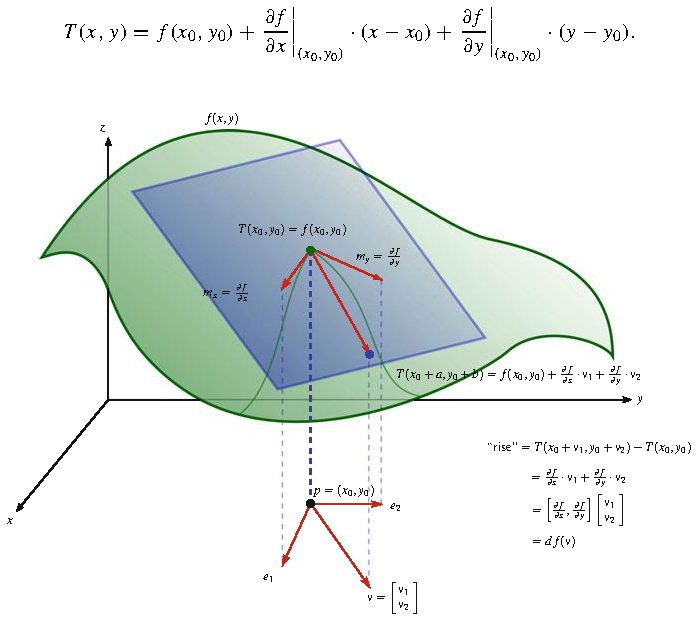
\includegraphics[width=0.960\linewidth]{images/vector/fig-2-31.pdf}
  \caption{微分 $df_p$ 是函数 $f$ 在点 $p$ 处的线性逼近. 换句话说, 微分 $df_p$``编码''了 $f$ 在 $p$ 处的切平面}
  \label{fig:2-31}
\end{figure}

如图所表明的, 给定向量 $v=\binom{v_1}{v_2}_p$, 这个向量的终点（在 $\mathbb{R}^2$ 中）是 $(x_0+v_1,y_0+v_2)$. $f$ 的切平面（在点 $p=(x_0,y_0)$ 处）中位于 $(x_0+v_1,y_0+v_2)$ 正上方的点由
\begin{align*}
T(x_0+v_1,y_0+v_2)
&=f(x_0,y_0)+\left.\frac{\partial f}{\partial x}\right|_{(x_0,y_0)}\cdot(x_0+v_1-x_0)+\left.\frac{\partial f}{\partial y}\right|_{(x_0,y_0)}\cdot(y_0+v_2-y_0)\\
&=f(x_0,y_0)+\left.\frac{\partial f}{\partial x}\right|_{(x_0,y_0)}\cdot v_1+\left.\frac{\partial f}{\partial y}\right|_{(x_0,y_0)}\cdot v_2
\end{align*}
给出, 所以切平面中从 $f(x_0,y_0)$ 起的``rise''由
\begin{align*}
\text{``rise''}&=T(x_0+v_1,y_0+v_2)-T(x_0,y_0)\\
&=f(x_0,y_0)+\left.\frac{\partial f}{\partial x}\right|_{(x_0,y_0)}\cdot v_1+\left.\frac{\partial f}{\partial y}\right|_{(x_0,y_0)}\cdot v_2-f(x_0,y_0)\\
&=\left.\frac{\partial f}{\partial x}\right|_{(x_0,y_0)}\cdot v_1+\left.\frac{\partial f}{\partial y}\right|_{(x_0,y_0)}\cdot v_2\\
&=df_p(v_p)
\end{align*}
给出. 因此, $f$ 在 $p$ 处的微分 $df_p$ 给出当你沿着向量 $v_p$ 移动时 $f$ 在 $p$ 处切平面的``rise'', 它本质上编码了这个切平面如何行为. 切平面是 $f$ 在 $p$ 处最接近的线性逼近, 所以本质上 $df_p$ 可以被想成函数 $f$ 在点 $p$ 处的线性逼近.

作为最后一个评注, 写成行向量的微分 1-形式 $df$
\[
df=\frac{\partial f}{\partial x}dx+\frac{\partial f}{\partial y}dy=\left(\frac{\partial f}{\partial x},\frac{\partial f}{\partial y}\right)
\]
（在 $\mathbb{R}^2$ 情形中）或
\[
df=\frac{\partial f}{\partial x}dx+\frac{\partial f}{\partial y}dy+\frac{\partial f}{\partial z}dz=\left(\frac{\partial f}{\partial x},\frac{\partial f}{\partial y},\frac{\partial f}{\partial z}\right)
\]
（在 $\mathbb{R}^3$ 情形中）是否让你想起向量微积分中的什么东西？它应该让你想起 $\mathrm{grad}(f)$ 或 $\nabla(f)$. 事实上, $df$ 和 $\mathrm{grad}(f)$ 密切相关. 我们将在第 9 章探讨这一关系.

我们现在考虑几个例子. 设 $f:\mathbb{R}^3\to\mathbb{R}$ 由 $f(x,y,z)=x^2y^3z$ 给出, 并考虑每个点 $p=(x,y,z)\in\mathbb{R}^3$ 处的向量 $v_p=\begin{bmatrix}1\\2\\3\end{bmatrix}_p$. 首先求 $df(v_p)$. 由于 $v_p$ 在每个点 $p$ 都相同, 我们可以从记号中略去 $p$. 我们有
\begin{align*}
df(v)&=v[f]\\
&=\left(\frac{\partial}{\partial x}+2\frac{\partial}{\partial y}+3\frac{\partial}{\partial z}\right)\left(x^2y^3z\right)\\
&=\frac{\partial(x^2y^3z)}{\partial x}+2\frac{\partial(x^2y^3z)}{\partial y}+3\frac{\partial(x^2y^3z)}{\partial z}\\
&=2xy^3z+2(3x^2y^2z)+3(x^2y^3).
\end{align*}
现在假设我们给定具体点 $p=(-1,2,-2)$. 在 $p=(-1,2,-2)$ 处求 $df(v_p)$ 只需要代入数值
\[
df(v_p)=2(-1)^2(2)^3(-2)+2\bigl(3(-1)^2(2)^2(-2)\bigr)+3(-1)^2(2)^3=8.
\]

\begin{question}\label{q:2-15}
设 $f(x,y,z)=(x^2-1)y+(y^2+2)z$.
\begin{enumerate}
  \item[(i)] 求 $df$.
  \item[(ii)] 令 $v_p=\begin{bmatrix}v_1\\v_2\\v_3\end{bmatrix}_{(p_1,p_2,p_3)}$. 求 $df(v_p)$.
  \item[(iii)] 令 $v_p=\begin{bmatrix}-2\\1\\3\end{bmatrix}_{(-1,0,2)}$. 求 $df(v_p)$.
\end{enumerate}
\end{question}

\begin{question}\label{q:2-16}
设 $f$ 和 $g$ 是 $\mathbb{R}^3$ 上的函数. 证明 $d(fg)=gdf+fdg$.
\end{question}

\begin{question}\label{q:2-17}
设 $f:\mathbb{R}^3\to\mathbb{R}$、$h:\mathbb{R}\to\mathbb{R}$ 和 $h(f):\mathbb{R}^3\to\mathbb{R}$ 都有定义. 证明 $d(h(f))=h'(f)df$.
\end{question}

\section{小结、参考文献与问题}

\subsection{小结}

因为这一区别对更抽象的空间很重要, 我们首先大谈特谈 $\mathbb{R}^n$ 中点的集合是流形 $\mathbb{R}^n$, 而 $\mathbb{R}^n$ 中向量的集合是向量空间 $\mathbb{R}^n$. 然后我们定义了笛卡尔函数 $x_i:\mathbb{R}^n\to\mathbb{R}$, 它把流形 $\mathbb{R}^n$ 中的点 $p$ 送到其第 $i$ 个坐标值.

$n$ 维流形 $M$ 在点 $p\in M$ 处的切空间被引入为 $M$ 在点 $p$ 处所有切向量的空间, 记为 $T_pM$. 切空间 $T_pM$ 本质上可以被看作附着在 $M$ 的点 $p$ 处的向量空间 $\mathbb{R}^n$ 的一个副本. 流形的所有切空间的集合称为切丛, 记为 $TM$. 向量场被定义为一个函数 $v$, 它给 $M$ 的每个点 $p$ 指派 $T_pM$ 的一个元素 $v_p$. 向量场有时被称为切丛的截面.

函数 $f:M\to\mathbb{R}$ 在点 $p$ 处沿方向 $v_p$ 的方向导数被定义为
\[
v_p[f]\equiv\left.\frac{d}{dt}f(p+tv_p)\right|_{t=0},
\]
这与向量微积分中的定义完全相同, 只是去掉了 $v_p$ 必须是单位向量的要求. 去掉这一要求略微改变了方向导数的几何意义, 但使我们能够保留简单的公式
\[
v_p[f]=\sum_{i=1}^{n}v_i\cdot\left.\frac{\partial f}{\partial x_i}\right|_{p_i}\qquad\text{其中}\qquad
v_p=\begin{bmatrix}v_1\\v_2\\\vdots\\v_n\end{bmatrix}.
\]
这个公式随后被用来做出最有用和最出人意料的等同之一, 
\begin{center}
\fbox{\parbox{0.86\textwidth}{\centering
欧几里得向量 $e_i$ 可以与偏微分算子 $\dfrac{\partial}{\partial x_i}$ 等同
}}
\end{center}
换句话说, 我们把欧几里得向量 $e_i$ 想成就是偏微分算子 $\frac{\partial}{\partial x_i}$.

这个方向导数随后被用来定义与函数 $f$ 相联系的一个特定线性泛函, 
\[
df(v_p)=v_p[f].
\]
这个线性泛函称为 $f$ 的微分. 由于 $v_p\in T_pM$, 而 $T_pM$ 是一个向量空间, 线性泛函 $df$ 在 $T_pM$ 的对偶空间中, 这个对偶空间称为余切空间. 我们写 $df\in T_p^*M$. 此外, 可以用笛卡尔坐标函数 $x_i$ 定义微分 $dx_i$, 事实证明它们是与 $T_pM$ 的欧几里得基对偶的 $T_p^*M$ 的基. 因此, 利用上面的等同, 我们有 $\{\frac{\partial}{\partial x_1},\ldots,\frac{\partial}{\partial x_n}\}$ 作为 $T_pM$ 的标准基, $\{dx_1,\ldots,dx_n\}$ 作为 $T_p^*M$ 的标准对偶基. $T_p^*M$ 的元素也称为微分 1-形式. 微分 1-形式 $dx_i$ 的行为类似于笛卡尔坐标函数, 挑出向量 $v_p$ 的第 $i$ 个分量, 即 $dx_i(v_p)=v_i$. 在几何上, 我们可以把 $dx_i$ 想成求 $v_p$ 在第 $i$ 个轴上的投影向量的长度.

\subsection{参考文献与进一步阅读}

向量和向量场出现在多元微积分的各个角落, 例如见 Stewart~\cite{ref43}, 甚至 Marsden 和 Hoffman~\cite{ref31}, 但切空间和切丛通常不会在这一层次遇到或明确化. 那通常留给更高级的课程, 常常是微分几何. 对这一材料有相当多有趣而严谨的导引. 仅举几例, Munkres~\cite{ref35}、O'Neill~\cite{ref36}、Tu~\cite{ref46}、Spivak~\cite{ref41} 和 Thorpe~\cite{ref45} 都是流形上分析与微分几何的好导引, 因此都包含关于切空间和切丛的出色论述. 同样, Stewart~\cite{ref43} 和 Marsden 与 Hoffman~\cite{ref31} 是方向导数和多元微积分的优秀参考书. 本章还通过考察微分 1-形式, 开始了对微分形式的温和导引, 这将用几章来完成. 本章关于微分 1-形式的材料大体上遵循了 Bachman~\cite{ref04} 和 O'Neill~\cite{ref36} 的精神, 不过也参考了 Munkres~\cite{ref35}、Edwards~\cite{ref18} 和 Martin~\cite{ref33}.

\subsection{问题}

\begin{question}\label{q:2-18}
令 $p_1=(2,9,-2)$、$p_2=(1,0,-3)$、$p_3=(12,-7,4)$ 是 $\mathbb{R}^3$ 中的点, 令 $x,y,z$ 是 $\mathbb{R}^3$ 上的笛卡尔坐标函数. 求
\begin{gather*}
\text{a) }x(p_1),\quad \text{d) }x(p_2),\quad \text{g) }x(p_3),\\
\text{b) }y(p_1),\quad \text{e) }y(p_2),\quad \text{h) }y(p_3),\\
\text{c) }z(p_1),\quad \text{f) }z(p_2),\quad \text{i) }z(p_3).
\end{gather*}
\end{question}

\begin{question}\label{q:2-19}
考虑流形 $\mathbb{R}^3$ 和向量场 $v=xye_1+\bigl(z-x^3\bigr)e_2-(x+z-4)e_3$, 其中 $e_1,e_2,e_3$ 是欧几里得向量. 若 $p_1=(1,-3,2)$、$p_2=(0,1,4)$、$p_3=(-5,-2,2)$, 求向量 $v_{p_1},v_{p_2},v_{p_3}$. 这些向量各在什么空间中？
\end{question}

\begin{question}\label{q:2-20}
求 $f(x,y)=5x^2y-4xy^3$ 在方向 $v_1=\binom{5}{12}$ 和 $v_2=\frac{1}{13}\binom{5}{12}$ 上、在点 $(1,2)$ 处的方向导数. 解释 $D_{v_1}f$ 与 $D_{v_2}f$ 之间的差别.
\end{question}

\begin{question}\label{q:2-21}
求 $f(x,y)=x\ln(y)$ 在方向 $v_1=\binom{-4}{3}$ 和 $v_2=\frac{1}{5}\binom{-4}{3}$ 上、在点 $(1,-3)$ 处的方向导数. 解释 $D_{v_1}f$ 与 $D_{v_2}f$ 之间的差别.
\end{question}

\begin{question}\label{q:2-22}
求 $f(x,y,z)=xe^{yz}$ 在方向 $v_1=\begin{bmatrix}2\\-2\\1\end{bmatrix}$ 和 $v_2=\frac{1}{3}\begin{bmatrix}2\\-2\\1\end{bmatrix}$ 上、在点 $(3,0,2)$ 处的方向导数. 解释 $D_{v_1}f$ 与 $D_{v_2}f$ 之间的差别.
\end{question}

\begin{question}\label{q:2-23}
给定 $f(x,y,z)=\sqrt{x+yz}$ 和 $v=2\frac{\partial}{\partial x}+3\frac{\partial}{\partial y}+6\frac{\partial}{\partial z}$, 求 $v[f]$ 在点 $(1,3,1)$ 处的值.
\end{question}

\begin{question}\label{q:2-24}
给定 $f(x,y,z)=xe^y+ye^z+ze^x$ 和 $v=5\frac{\partial}{\partial x}+1\frac{\partial}{\partial y}-2\frac{\partial}{\partial z}$, 求 $v[f]$ 在点 $(0,0,0)$ 处的值.
\end{question}

\begin{question}\label{q:2-25}
给定 $f(x,y,z)=\sqrt{xyz}$ 和 $v=-1\frac{\partial}{\partial x}-2\frac{\partial}{\partial y}+2\frac{\partial}{\partial z}$, 求 $v[f]$ 在点 $(3,2,6)$ 处的值.
\end{question}

\begin{question}\label{q:2-26}
给定 $f(x,y,z)=x+y^2+z^3$ 和 $v=-3\frac{\partial}{\partial x}+4\frac{\partial}{\partial y}-2\frac{\partial}{\partial z}$, 求 $v[f]$ 在点 $(2,5,-1)$ 处的值.
\end{question}

\begin{question}\label{q:2-27}
给定流形 $\mathbb{R}^3$ 上的 1-形式 $\alpha=(x^3+2yz^2)dx+(xy-2)dy+x^4dz$, 对 $p_1=(-1,3,2)$、$p_2=(2,-2,1)$、$p_3=(3,-5,-2)$ 求 1-形式 $\alpha_{p_i}$.
\end{question}

\begin{question}\label{q:2-28}
给定流形 $\mathbb{R}^3$ 上的 1-形式 $\alpha=(x^3-2yz^2)dx+dy+x^4dz$, 对 $p_1=(-1,3,2)$、$p_2=(2,-2,1)$、$p_3=(3,-5,-2)$ 求 1-形式 $\alpha_{p_i}$.
\end{question}

\begin{question}\label{q:2-29}
给定 $\mathbb{R}^3$ 上的 1-形式 $\alpha=(x^3+2yz^2)dx+(xy-2)dy+x^4dz$ 和 $\beta=(x^3-2yz^2)dx+dy+x^4dz$, 求 1-形式 $\alpha+\beta$ 和 $\alpha-\beta$. 然后对上一题中的点 $p_i$ 求 $(\alpha+\beta)_{p_i}$ 和 $(\alpha-\beta)_{p_i}$.
\end{question}

\begin{question}\label{q:2-30}
给定 1-形式 $\alpha=x^3dx-xyzdy+y^2dz$, 求 1-形式 $2\alpha$ 和 $\frac13\alpha$.
\end{question}

\begin{question}\label{q:2-31}
给定 1-形式 $\omega=\frac{xy}{2}dx-\sqrt{yz}dy+(x+z)^\frac23dz$ 和 $p=(2,-1,3)$, 对下列向量求 $\alpha_p(v_p)$：
\begin{enumerate}
  \item[(a)] $\begin{bmatrix}2\\-2\\1\end{bmatrix}$
  \item[(b)] $\begin{bmatrix}1\\3\\-5\end{bmatrix}$
  \item[(c)] $\begin{bmatrix}x+y\\z-2\\xz\end{bmatrix}$
  \item[(d)] $4e_1+7e_2-3e_3$
  \item[(e)] $\frac12e_1+\frac74e_2-\frac35e_3$
  \item[(f)] $-\sqrt{xy}e_1+\sqrt{xz}e_2-3ye_3$
  \item[(g)] $2\frac{\partial}{\partial x}-3\frac{\partial}{\partial y}+4\frac{\partial}{\partial z}$
  \item[(h)] $-2\frac{\partial}{\partial x}+\frac53\frac{\partial}{\partial y}+\frac{\partial}{\partial z}$
  \item[(i)] $\sqrt{x+y+z}\frac{\partial}{\partial x}-\sqrt{x}\ln(y)\frac{\partial}{\partial y}+\sqrt{zy}\frac{\partial}{\partial z}$
\end{enumerate}
\end{question}

\begin{question}\label{q:2-32}
求下列函数的微分 $df$：
\begin{enumerate}
  \item[(a)] $f(x,y)=x^2y^3$
  \item[(b)] $f(x,y)=x^2+y^2$
  \item[(c)] $f(x,y)=x+y^3$
  \item[(d)] $f(x,y,z)=x^2+y^3+z^4$
  \item[(e)] $f(x,y,z)=\sqrt{xyz}$
  \item[(f)] $f(x,y,z)=xe^y+ye^z+ze^x$
  \item[(g)] $f(x,y,z)=\sqrt{x+yz}$
  \item[(h)] $f(x,y,z)=x\ln(y)+y\ln(z)+z\ln(x)$
  \item[(i)] $f(x,y,z)=\left(x^3+y^3+z^3\right)^\frac23$
\end{enumerate}
\end{question}

\begin{question}\label{q:2-33}
对你在上一题中求出的微分以及上一题之前的题中的向量, 在点 $p=(2,-1,3)$ 处求 $df[v_p]$.
\end{question}
